
%----------------------------------------------------------------------------------------
%	PART
%----------------------------------------------------------------------------------------
\part{Capítulo siete}
% \spanishdecimal{.}
\graphicspath{ {7_Capitulo/img/ejemplos/}, {W_Varios/2_Portada_capitulos/} }

%----------------------------------------------------------------------------------------
%	CHAPTER 7
%----------------------------------------------------------------------------------------

\chapterimage{ima2} % Chapter heading image


\chapter{Amortización y Capitalización}

%\begin{center}
%    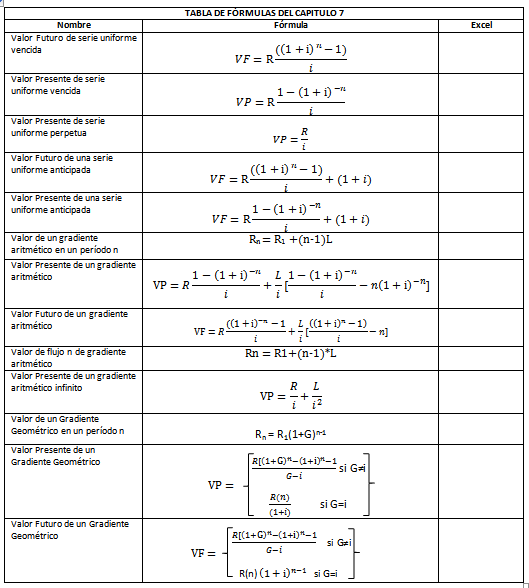
\includegraphics[scale=1]{7_0}
%\end{center}

\section{Mapa Mental}
\begin{center}
	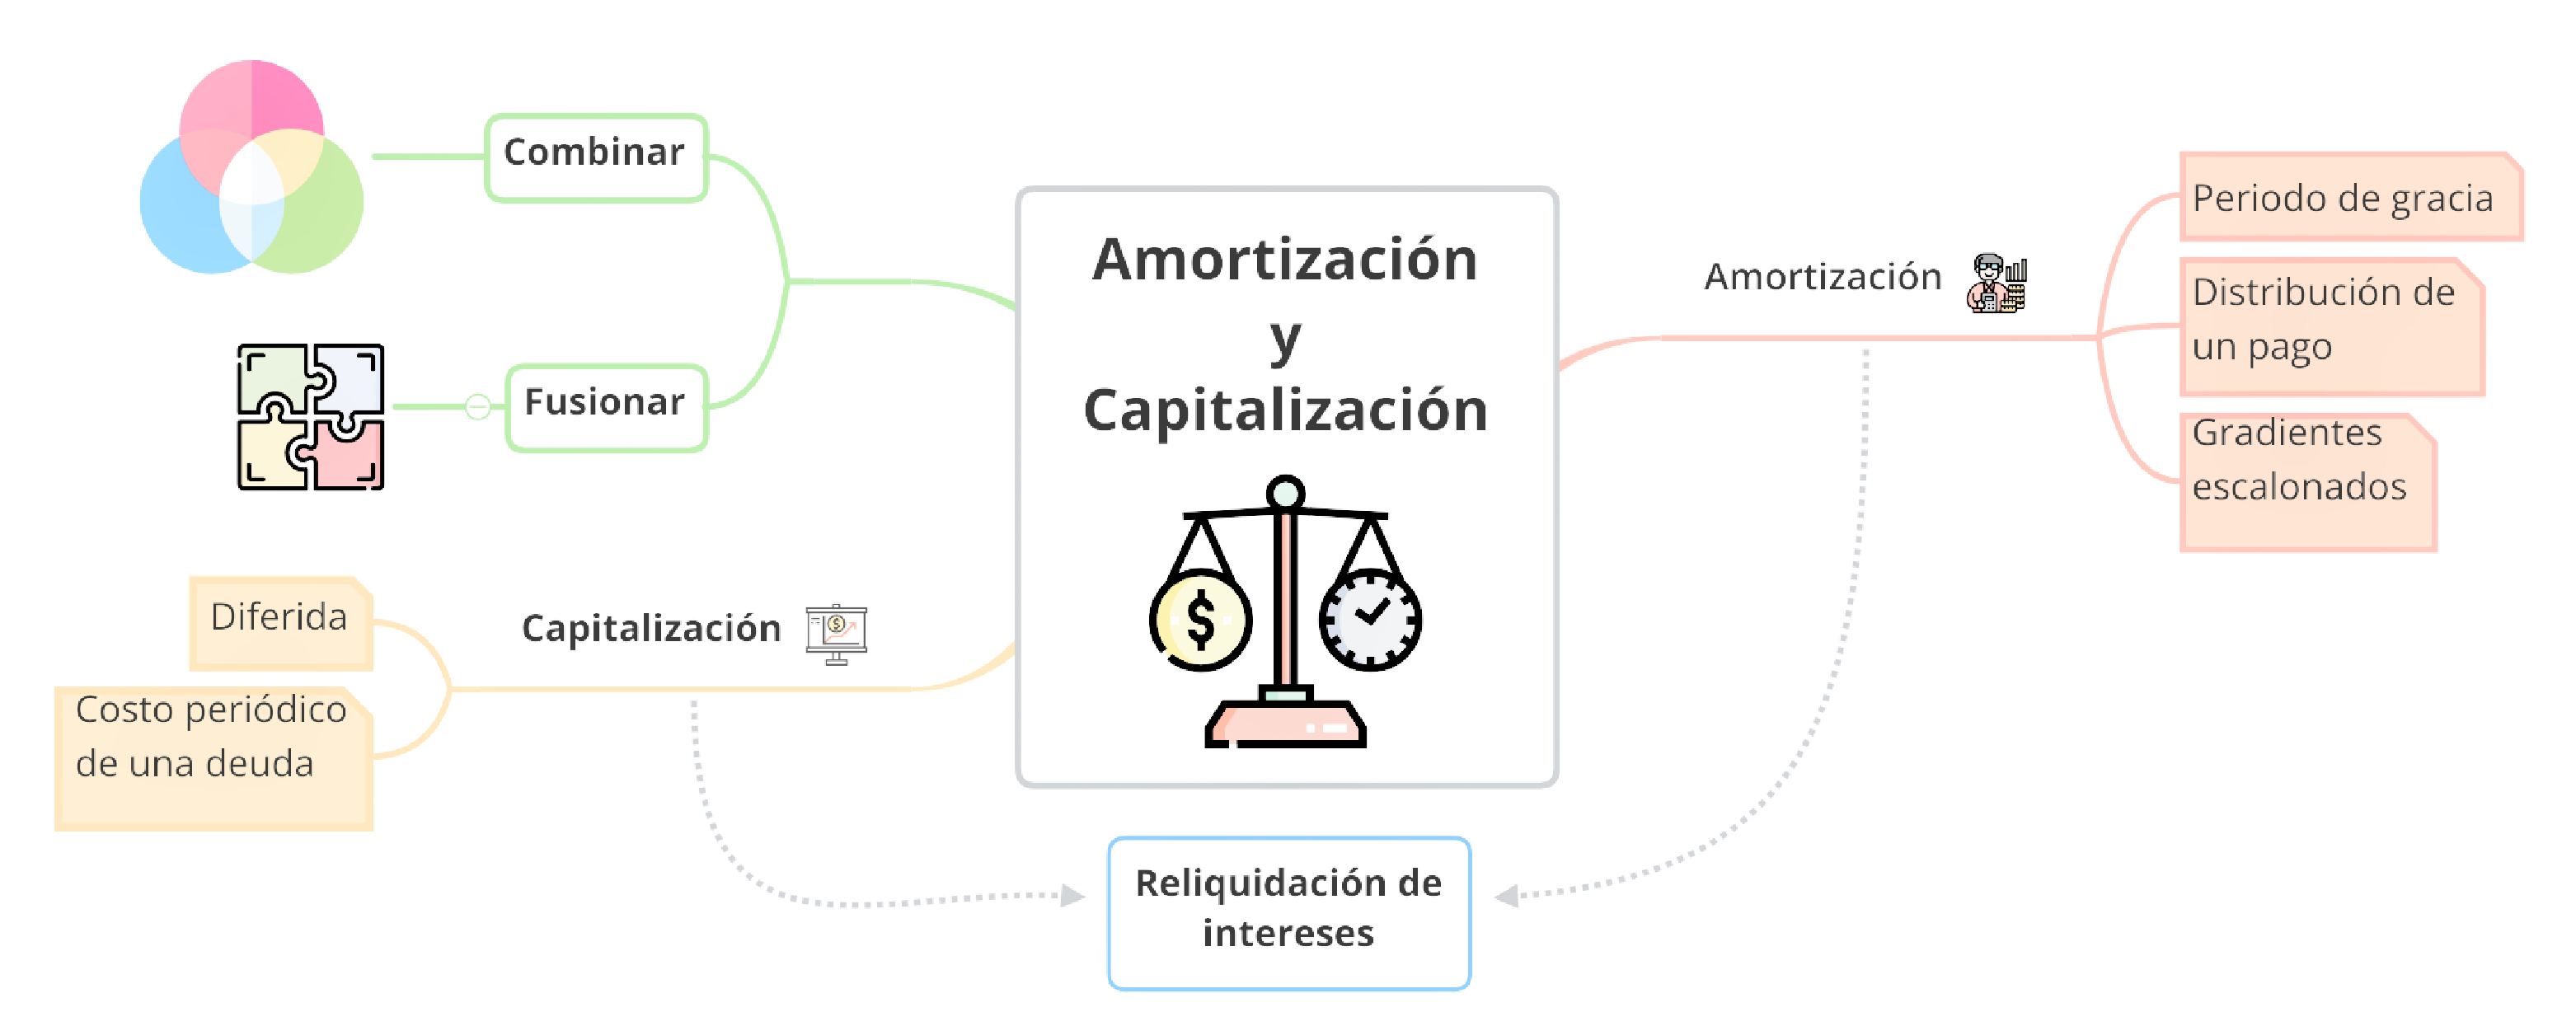
\includegraphics[scale=0.30]{7_Capitulo/img/explicacion/Mapa Mental 7.pdf}
\end{center}

\section{Introducción del capítulo}

Uno de los aspectos más importantes en las finanzas es la amortización, porque es la forma más fácil de pagar una deuda; como también lo es la capitalización, porque así podremos reunir un capital mediante ahorros periódicos. El objetivo en ambos casos viene a ser la financiación de un proyecto. Una manera de visualizar mejor el flujo de caja y el comportamiento de la deuda o del capital a través del tiempo, es mediante el uso de tablas.


\section{Amortización de cuotas con reliquidación de intereses}

Son aquellas en las que deudor y acreedor acuerdan las fechas en que se van a efectuar tales cuotas extraordinarias en el mismo momento en que se contrata el crédito.\\

%%%%%%%%%%%%%%%%%%% EJERCICIO 1 %%%%%%
\textbf{Ejemplo 1:}\\

Se va a cancelar una deuda por 200.000 COP en 4 pagos trimestrales de R COP cuota ordinaria, con una tasa de interés de 32\% nominal anual trimestre vencido. Hallar el valor de las cuotas ordinarias.\\

%%%%%%%%%%%%%%%%%%% EJERCICIO 1a %%%%%%

%\newpage %USAR SOLO SI EL SOLUCIÓN QUEDA SOLO Y ES NECESARIO BAJARLO A LA SIGUIENTE PAGINA
\textbf{Solución.}\\
%La tabla ira centrada
\begin{center}
	\renewcommand{\arraystretch}{1.6}% Margenes de las celdas
	%Creación de la cuadricula de 3 columnas
	\begin{longtable}[H]{|c|c|c|}
		%Creamos una linea horizontal
		\hline
		%Definimos el color de la primera fila
		\rowcolor[HTML]{FFB183}
		%%%%% INICIO ASIGNACIÓN PERIODO FOCAL %%%%%%%
		%%%%%%%%%% INICIO TITULO
		%Lo que se hace aquí es mezclar las 3 columnas en una sola
		\multicolumn{3}{|c|}{\cellcolor[HTML]{FFB183}\textbf{1. Asignación período focal}}  \\ \hline
		\multicolumn{3}{|c|}{$pf : \textit{0 ptv}$}   \\\hline
		%%%%%%%%%% FIN TITULO
		%%%%% INICIO DECLARACIÓN DE VARIABLES %%%%%%%
		%%%%%%%%%% INICIO TITULO
		%Lo que se hace aquí es mezclar las 3 columnas en una sola
		\multicolumn{3}{|c|}{\cellcolor[HTML]{FFB183}\textbf{2. Declaración de variables}}   \\ \hline
		%%%%%%%%%% FIN TITULO
		%%%%%%%%%% INICIO DE MATEMÁTICAS
		%Cada & hace referencia al paso de la siguiente columna

		\cellcolor[HTML]{FFB183}\textbf{Valores monetarios} & 
		\cellcolor[HTML]{FFB183}\textbf{Valores no monetarios} & 
		\cellcolor[HTML]{FFB183}\textbf{Incógnitas}  \\ \hline
	 	$ \hspace{1cm} VP= 200{.}000 \ COP \hspace{1cm}$ & $\hspace{1.5cm} i = 8\% \ \textit{ptv} \hspace{1.5cm}$ & $R=\textit{?COP} $ \\
		& $ n=\textit{4 ptv} $ &  \\
		& $ j = 32\% \ \textit{natv} $ &  \\ \hline
	

		%%%%%%%%%% FIN DE MATEMÁTICAS
		%%%%% FIN DECLARACIÓN DE VARIABLES
		
		
		%%%%% INICIO FLUJO DE CAJA
		\rowcolor[HTML]{FFB183}
		\multicolumn{3}{|c|}{\cellcolor[HTML]{FFB183}\textbf{3. Diagrama de flujo de caja}} \\ \hline
		%Mezclamos 3 columnas y pondremos el dibujo
		%%%%%%%%%%%%% INSERCIÓN DE LA IMAGEN
		%Deberán descargar las imágenes respectivas del drive y pegarlas en la carpeta
		%n_capitulo/img/ejemplos/1/capitulo1ejemplo1.pdf  (el /1/ es el numero del ejemplo)
		\multicolumn{3}{|c|}{ 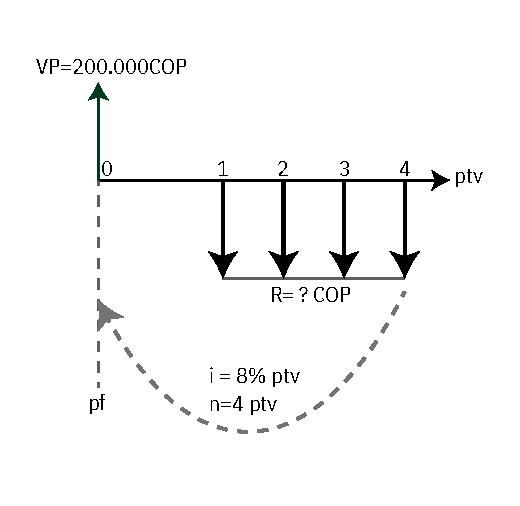
\includegraphics[trim=-78 -5 -78 -5]{7_Capitulo/img/ejemplos/1/Capitulo7-Ejercicio1.pdf} }
		
		
		\\ \hline
		%%%%%%%%%%%%% FIN INSERCIÓN DE IMAGEN
		%%%%%FIN FLUJO DE CAJA
		
		
		
		%%%%% INICIO DECLARACIÓN FORMULAS
		%%%%%%%%%%% INICIO TITULO
		\rowcolor[HTML]{FFB183}
		\multicolumn{3}{|c|}{\cellcolor[HTML]{FFB183}\textbf{4. Declaración de fórmulas}}    \\ \hline
		%%%%%%%%%%% FIN TITULO
		%%%%%%%%%%% INICIO MATEMÁTICAS
		
		\multicolumn{3}{|c|}{$VP=R(\frac{1-(1+i)^{-n}}{i}) \hspace{0.4 cm} \textit{Valor presente de una serie uniforme vencida}$} \\ \hline
		
		%%%%%%%%%% FIN MATEMÁTICAS
		%%%%%% INICIO DESARROLLO MATEMÁTICO
		\rowcolor[HTML]{FFB183}
		%%%%%%%%%%INICIO TITULO
		\multicolumn{3}{|c|}{\cellcolor[HTML]{FFB183}\textbf{5. Desarrollo matemático}}       \\ \hline
		%%%%%%%%%% FIN TITULO
		%%%%%%%%%% INICIO MATEMÁTICAS
		\multicolumn{3}{|c|}{$ 200{.}000 \ COP=R(\frac {1-(1+0.08)^{-4}} {0.08}) $ \hspace{0.2 cm} $\rightarrow$ \hspace{0.2 cm} $ R= 60{.}384.16 \ COP $} \\ \hline
		
		%%%%%%%%%% FIN MATEMÁTICAS
		%%%%%% FIN DESARROLLO MATEMÁTICO
		%%%%%% INICIO RESPUESTA
		\rowcolor[HTML]{FFB183}
		%%%%%%%%%%INICIO TITULO
		\multicolumn{3}{|c|}{\cellcolor[HTML]{FFB183}\textbf{6. Respuesta}}   \\ \hline
		%%%%%%%%%% FIN TITULO
		%%%%%%%%%% INICIO RESPUESTA MATEMÁTICA
		\multicolumn{3}{|c|}{$\mathbf{R= 60{.}384.16 \ COP}$}
		\begin{comment}
		\multicolumn{3}{|p{\textwidth}|}{
		$F_{4} = F_{5} = 21.609,84 \ COP $ }
		\end{comment} 
		\\ \hline
		%%%%%%%%%% FIN MATEMÁTICAS
		%%%%%% FIN RESPUESTA
	\end{longtable}
	%Se crean dos lineas en blanco para que no quede el siguiente texto tan pegado
	%\newline \newline %USARLO SI CREES QUE ES NECESARIO
\end{center}
%%%%%%%%%%%%%%%%%%%%%%%%%%FIN EJERCICIO 1a %%%%%%%%%%%%%%%%%%%%%%%%%%%

%%%%%%%%%%%%%%%%%%% EJERCICIO 1b %%%%%%
Pero si se hace un pago adicional de 50.000 COP al final del noveno periodo mes vencido, la cuota ordinaria debe bajar porque al plantear la ecuación de valor se debe incluir un pago más y en este caso se dice que esa cuota es extra pactada y el diagrama de flujo de caja quedará así:\\
%\newpage %USAR SOLO SI EL SOLUCIÓN QUEDA SOLO Y ES NECESARIO BAJARLO A LA SIGUIENTE PAGINA
\textbf{Solución.}\\
%La tabla ira centrada
\begin{center}
	\renewcommand{\arraystretch}{1.5}% Margenes de las celdas
	%Creación de la cuadricula de 3 columnas
	\begin{longtable}[H]{|c|c|c|}
		%Creamos una linea horizontal
		\hline
		%Definimos el color de la primera fila
		\rowcolor[HTML]{FFB183}
		%%%%% INICIO ASIGNACIÓN PERIODO FOCAL %%%%%%%
		%%%%%%%%%% INICIO TITULO
		%Lo que se hace aquí es mezclar las 3 columnas en una sola
		\multicolumn{3}{|c|}{\cellcolor[HTML]{FFB183}\textbf{1. Asignación período focal}}  \\ \hline
		\multicolumn{3}{|c|}{$pf : \textit{0 ptv}$}   \\\hline
		%%%%%%%%%% FIN TITULO
		%%%%% INICIO DECLARACIÓN DE VARIABLES %%%%%%%
		%%%%%%%%%% INICIO TITULO
		%Lo que se hace aquí es mezclar las 3 columnas en una sola
		\multicolumn{3}{|c|}{\cellcolor[HTML]{FFB183}\textbf{2. Declaración de variables}}   \\ \hline
		%%%%%%%%%% FIN TITULO
		%%%%%%%%%% INICIO DE MATEMÁTICAS
		%Cada & hace referencia al paso de la siguiente columna
		\cellcolor[HTML]{FFB183}\textbf{Valores monetarios} & 
		\cellcolor[HTML]{FFB183}\textbf{Valores no monetarios} & 
		\cellcolor[HTML]{FFB183}\textbf{Incógnitas}  \\ \hline
	 	$ \hspace{1cm} VP= 200{.}000 \ COP \hspace{1cm}$ & $\hspace{1.5cm} i =  8\% \ \textit{ptv} \hspace{1.5cm}$ & $ R=\textit{?COP} $ \\
		$ \hspace{1cm} F = 50{.}000 \ COP \hspace{1cm}$ & $ n_1=\textit{4 ptv} $ &  \\
		& $ n_2=\textit{3 ptv} $ &  \\
		& $ j = 32\% \textit{natv} $ &  \\ \hline
		
		
		%%%%%%%%%% FIN DE MATEMÁTICAS
		%%%%% FIN DECLARACIÓN DE VARIABLES
		
		
		%%%%% INICIO FLUJO DE CAJA
		\rowcolor[HTML]{FFB183}
		\multicolumn{3}{|c|}{\cellcolor[HTML]{FFB183}\textbf{3. Diagrama de flujo de caja}} \\ \hline
		%Mezclamos 3 columnas y pondremos el dibujo
		%%%%%%%%%%%%% INSERCIÓN DE LA IMAGEN
		%Deberán descargar las imágenes respectivas del drive y pegarlas en la carpeta
		%n_capitulo/img/ejemplos/1/capitulo1ejemplo1.pdf  (el /1/ es el numero del ejemplo)
		\multicolumn{3}{|c|}{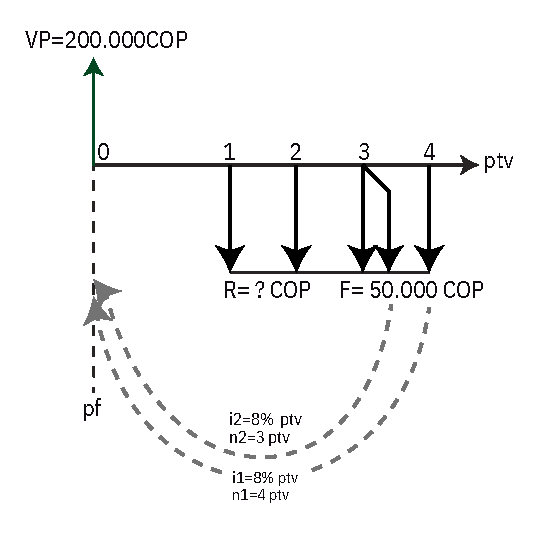
\includegraphics[trim=-78 -5 -78 -5]{7_Capitulo/img/ejemplos/1/Capitulo7Ejercicio1b.pdf} }
		
		
		\\ \hline
		%%%%%%%%%%%%% FIN INSERCIÓN DE IMAGEN
		%%%%%FIN FLUJO DE CAJA
		
		
		
		%%%%% INICIO DECLARACIÓN FORMULAS
		%%%%%%%%%%% INICIO TITULO
		\rowcolor[HTML]{FFB183}
		\multicolumn{3}{|c|}{\cellcolor[HTML]{FFB183}\textbf{4. Declaración de fórmulas}}    \\ \hline
		%%%%%%%%%%% FIN TITULO
		%%%%%%%%%%% INICIO MATEMÁTICAS
		\multicolumn{3}{|c|}{$P=F(1+i)^{-n} \hspace{0.4 cm} \textit{Valor presente dado de un valor futuro}$} \\
		\multicolumn{3}{|c|}{$VP=R(\frac{1-(1+i)^{-n}}{i}) \hspace{0.4 cm} \textit{Valor presente de una serie uniforme vencida}$} \\ \hline
		
		%%%%%%%%%% FIN MATEMÁTICAS
		%%%%%% INICIO DESARROLLO MATEMÁTICO
		\rowcolor[HTML]{FFB183}
		%%%%%%%%%%INICIO TITULO
		\multicolumn{3}{|c|}{\cellcolor[HTML]{FFB183}\textbf{5. Desarrollo matemático}}       \\ \hline
		%%%%%%%%%% FIN TITULO
		%%%%%%%%%% INICIO MATEMÁTICAS
		\multicolumn{3}{|c|}{$ 200{.}000 \ COP =R(\frac{1-(1+0.08)^{-4}}{0.08})+ 50{.}000 \ COP (1+ 0.08)^{-4}\hspace{0.2 cm}\rightarrow \hspace{0.2 cm}R= 48{.}400.44 \ COP$} \\ \hline
		
		%%%%%%%%%% FIN MATEMÁTICAS
		%%%%%% FIN DESARROLLO MATEMÁTICO
		%%%%%% INICIO RESPUESTA
		\rowcolor[HTML]{FFB183}
		%%%%%%%%%%INICIO TITULO
		\multicolumn{3}{|c|}{\cellcolor[HTML]{FFB183}\textbf{6. Respuesta}}   \\ \hline
		%%%%%%%%%% FIN TITULO
		%%%%%%%%%% INICIO RESPUESTA MATEMÁTICA
		\multicolumn{3}{|c|}{$\mathbf{R= 48{.}400.44 \ COP}$}
		\begin{comment}
		\multicolumn{3}{|p{\textwidth}|}{
		$F_{4} = F_{5} = 21.609,84 \ COP $ .}
		\end{comment} 
		\\ \hline
		%%%%%%%%%% FIN MATEMÁTICAS
		%%%%%% FIN RESPUESTA
	\end{longtable}
	%Se crean dos lineas en blanco para que no quede el siguiente texto tan pegado
	%\newline \newline %USARLO SI CREES QUE ES NECESARIO
\end{center}
%%%%%%%%%%%%%%%%%%%%%%%%%%FIN EJERCICIO 1b %%%%%%%%%%%%%%%%%%%%%%%%%%%

Al elaborar la tabla de amortización, se debe tener presente que en el período 3 el valor del pago debe ser igual al pago ordinario más el pago extraordinario, tal como se ve en la siguiente tabla:\\


\begin{spacing}{1.1}
	%\begin{center}
    \footnotesize
	\begin{tabular}{|p{1cm}|p{3cm}|p{3cm}|p{3cm}|p{3cm}|}
		\hline
		\textbf{PER\ (1)} & \textbf{SALDO DEUDA (2)=(2)-(5)} & \textbf{INTERESES  (3)=(2)(i)} & \textbf{PAGO\ (4)=R COP - L COP} & \textbf{AMORTIZACIÓN  (5)=(4)-(3)} \\ \hline                    0 &   200.000,00 \ COP & --------- & --------- & ---------\\ \hline
		1                 &  167.599,56 \ COP                     &  16.000,00 \ COP                    &   48.400,44 \ COP                &  32.400,44 \ COP                        \\ \hline
		2                 &  132.609,08 \ COP                     &   13.407,96 \ COP                    &   48.400,44 \ COP                 &  34.992,48 \ COP                        \\ \hline
		3                 &  44.815,21 \ COP                      &  10.608,57 \ COP                     &  \textbf{98.400,44 \ COP }                  &  87.791,87 \ COP                        \\ \hline
		4                 &  0,00 \ COP                           &  3.585,23 \ COP                      &   48.400,44 \ COP                &  44.815,21 \ COP                        \\ \hline
	\end{tabular}
	%\end{center}
\end{spacing}
%%%%%%%%%%%%%%%%%%%%%%%%%%FIN EJERCICIO 1 %%%%%%%%%%%%%%%%%%%%%%%%%%%

\section{Amortización de cuotas sin reliquidación de intereses }
Cuando se está realizando una amortización y el deudor desea hacer un abono extra que no se había convenido en un principio al obtener el crédito, en este caso se dice que la cuota extra es “no pactada”, es apenas lógico, que ésta cuota no aparecerá en la ecuación de valor inicial porque no se había pactado inicialmente y se presentan dos situaciones, la primera opción consiste en abonarlo al saldo de su deuda y dejar que las cuotas ordinarias se sigan haciendo del mismo valor, en este caso la deuda se cancelará antes del plazo previsto, la segunda situación consiste en hacer el abono al saldo de la deuda y efectuar la reliquidación de la cuota ordinaria periódica con el fin de conservar el plazo originalmente pactado, claramente el valor de la nueva cuota ordinaria será inferior a la liquidada originalmente.
\\\\

%%%%%%%%%%%%%%%%%%% EJERCICIO 2 %%%%%%
%%%%%%%%%%%%%%%%%%% EJERCICIO 2a %%%%%%
\textbf{Ejemplo 2 }\\
Una deuda de  600.000 COP se va a cancelar en 7 pagos trimestrales con un interés del 9\% periódo trimestre vencido. Si al momento de efectuar el pago número 3 se efectúa un abono 2 extraordinario, no pactado, de 250.000 COP. Se pide: \\
a) Elaborar una tabla de amortización sin considerar el abono.\\
b) Elaborar una tabla suponiendo que la cuota extra se abona a capital sin reliquidar la cuota. \\
c) Elaborar una tabla de amortización si al hacer el abono extra se pide reliquidar la cuota.\\

%\newpage %USAR SOLO SI EL SOLUCIÓN QUEDA SOLO Y ES NECESARIO BAJARLO A LA SIGUIENTE PAGINA
\textbf{Solución.\\ a) }\\
%La tabla ira centrada
\begin{center}
	\renewcommand{\arraystretch}{1.5}% Margenes de las celdas
	%Creación de la cuadricula de 3 columnas
	\begin{longtable}[H]{|c|c|c|}
		%Creamos una linea horizontal
		\hline
		%Definimos el color de la primera fila
		\rowcolor[HTML]{FFB183}
		%%%%% INICIO ASIGNACIÓN PERIODO FOCAL %%%%%%%
		%%%%%%%%%% INICIO TITULO
		%Lo que se hace aquí es mezclar las 3 columnas en una sola
		\multicolumn{3}{|c|}{\cellcolor[HTML]{FFB183}\textbf{1. Asignación período focal}}  \\ \hline
		\multicolumn{3}{|c|}{$pf : \textit{0 ptv}$}   \\\hline
		%%%%%%%%%% FIN TITULO
		%%%%% INICIO DECLARACIÓN DE VARIABLES %%%%%%%
		%%%%%%%%%% INICIO TITULO
		%Lo que se hace aquí es mezclar las 3 columnas en una sola
		\multicolumn{3}{|c|}{\cellcolor[HTML]{FFB183}\textbf{2. Declaración de variables}}   \\ \hline
		%%%%%%%%%% FIN TITULO
		%%%%%%%%%% INICIO DE MATEMÁTICAS
		%Cada & hace referencia al paso de la siguiente columna
		\cellcolor[HTML]{FFB183}\textbf{Valores monetarios} & 
		\cellcolor[HTML]{FFB183}\textbf{Valores no monetarios} & 
		\cellcolor[HTML]{FFB183}\textbf{Incógnitas}  \\ \hline
	 	$ \hspace{1cm} VP= 600{.}000 \ COP \hspace{1cm}$ & $\hspace{1.5cm} i = 9\% \textit{ ptv} \hspace{1.5cm}$ & $ R = ? COP $ \\
		& $ n_1 = 7 \textit{ ptv} $ &  \\ \hline
		
		
		%%%%%%%%%% FIN DE MATEMÁTICAS
		%%%%% FIN DECLARACIÓN DE VARIABLES
		
		
		%%%%% INICIO FLUJO DE CAJA
		\rowcolor[HTML]{FFB183}
		\multicolumn{3}{|c|}{\cellcolor[HTML]{FFB183}\textbf{3. Diagrama de flujo de caja}} \\ \hline
		%Mezclamos 3 columnas y pondremos el dibujo
		%%%%%%%%%%%%% INSERCIÓN DE LA IMAGEN
		%Deberán descargar las imágenes respectivas del drive y pegarlas en la carpeta
		%n_capitulo/img/ejemplos/1/capitulo1ejemplo1.pdf  (el /1/ es el numero del ejemplo)
		\multicolumn{3}{|c|}{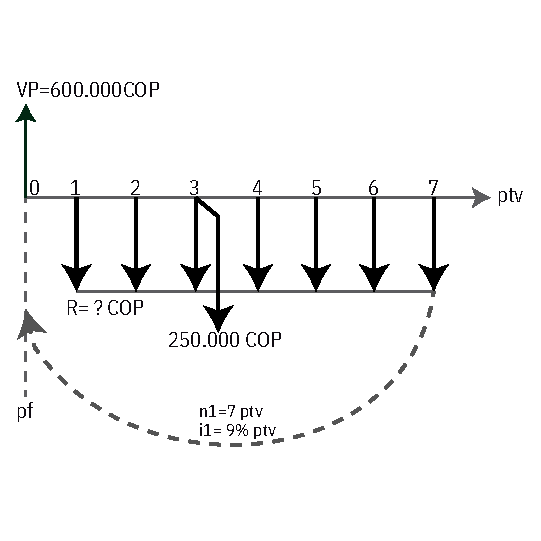
\includegraphics[trim=-78 -5 -78 -5]{7_Capitulo/img/ejemplos/2/Capitulo7Ejercicio2.pdf} }
		
		
		\\ \hline
		%%%%%%%%%%%%% FIN INSERCIÓN DE IMAGEN
		%%%%%FIN FLUJO DE CAJA
		
		
		
		%%%%% INICIO DECLARACIÓN FORMULAS
		%%%%%%%%%%% INICIO TITULO
		\rowcolor[HTML]{FFB183}
		\multicolumn{3}{|c|}{\cellcolor[HTML]{FFB183}\textbf{4. Declaración de fórmulas}}    \\ \hline
		%%%%%%%%%%% FIN TITULO
		%%%%%%%%%%% INICIO MATEMÁTICAS
		\multicolumn{3}{|c|}{$VP=R(\frac{1-(1+i)^{-n}}{i}) \hspace{0.4 cm} \textit{Valor presente de una serie uniforme vencida}$} \\ \hline
		
		%%%%%%%%%% FIN MATEMÁTICAS
		%%%%%% INICIO DESARROLLO MATEMÁTICO
		\rowcolor[HTML]{FFB183}
		%%%%%%%%%%INICIO TITULO
		\multicolumn{3}{|c|}{\cellcolor[HTML]{FFB183}\textbf{5. Desarrollo matemático}}       \\ \hline
		%%%%%%%%%% FIN TITULO
		%%%%%%%%%% INICIO MATEMÁTICAS
		\multicolumn{3}{|c|}{$ 600{.}000 \ COP =R(\frac{1-(1+0.09)^{-7}}{0.09})\hspace{0.2 cm}\rightarrow \hspace{0.2 cm}R= 119{.}214.31 \ COP$} \\ \hline
		
		%%%%%%%%%% FIN MATEMÁTICAS
		%%%%%% FIN DESARROLLO MATEMÁTICO
		%%%%%% INICIO RESPUESTA
		\rowcolor[HTML]{FFB183}
		%%%%%%%%%%INICIO TITULO
		\multicolumn{3}{|c|}{\cellcolor[HTML]{FFB183}\textbf{6. Respuesta}}   \\ \hline
		%%%%%%%%%% FIN TITULO
		%%%%%%%%%% INICIO RESPUESTA MATEMÁTICA
		\multicolumn{3}{|c|}{$\mathbf{R= 119{.}214.31 \ COP}$}
		\begin{comment}
		\multicolumn{3}{|p{\textwidth}|}{
		$F_{4} = F_{5} = 21.609,84 \ COP$ .}
		\end{comment} 
		\\ \hline
		%%%%%%%%%% FIN MATEMÁTICAS
		%%%%%% FIN RESPUESTA
	\end{longtable}
	%Se crean dos lineas en blanco para que no quede el siguiente texto tan pegado
	%\newline \newline %USARLO SI CREES QUE ES NECESARIO
\end{center}
%%%%%%%%%%%%%%%%%%%%%%%%%%FIN EJERCICIO 2a %%%%%%%%%%%%%%%%%%%%%%%%%%%
\newpage
Ahora elaboramos la tabla sin tener en cuenta ninguna cuota extra ya que no se han pactado.

\begin{spacing}{1.1}
	\begin{center}
        \footnotesize
		\begin{tabular}{|p{1cm}|p{2cm}|p{2cm}|p{2cm}|p{3cm}|}   
			\hline
			\textbf{PER\ (1)} & \textbf{SALDO DEUDA(2)=(2)-(5)} & \textbf{INTERESES  (3)=(2)(i)} & \textbf{PAGO(4)=COP R- COP L } & \textbf{AMORTIZACIÓN  (5)=(4)-(3)} \\ \hline
			
			0                 &   600.000 \ COP                     & ---------                       & ---------                   & ---------                          \\ \hline
			1                 &   534.785,69 \ COP                     &  54.000,00 \ COP                    &  119.214,31 \ COP                &  65.214,31 \ COP                        \\ \hline
			2                 &  463.702,09 \ COP                     &  48.130,71 \ COP                    &  119.214,31 \ COP                &    71.083,60 \ COP                        \\ \hline
			3                 &  386.220,97 \ COP                     &  41.733,19 \ COP                     &  119.214,31 \ COP                &   77.481,12 \ COP                        \\ \hline
			4                 &  301.766,55 \ COP                     &  34.759,88 \ COP                     &  119.214,31 \ COP                &  84.454,42 \ COP                        \\ \hline
			5                 &  209.711,23 \ COP                     &  27.158,99 \ COP                     &  119.214,31 \ COP                &   92.055,32 \ COP                        \\ \hline
			6                 &  109.370,93 \ COP                     &  18.874,01 \ COP                     &  119.214,31 \ COP                &  100.340,30 \ COP                       \\ \hline
			7                 &  0,00 \ COP                           &  9.843,38 \ COP                      &  119.214,31 \ COP                &  109.370,93 \ COP                       \\ \hline
		\end{tabular}
	\end{center}
\end{spacing}

La primera forma se puede presentar cuando, al cancelar la tercera cuota, el deudor decide efectuar un abono de 250.000 \ COP, adicional a su cuota ordinaria periódica, entonces la tabla quedará así:\\
\textbf{Solución.}\\
\textbf{b)}
\begin{spacing}{1.1}
	\begin{center}
    \footnotesize
		\begin{tabular}{|p{1cm}|p{2cm}|p{2cm}|p{2cm}|p{3cm}|}
			\hline
			\textbf{PER\ (1)} & \textbf{SALDO DEUDA(2)=(2)-(5)} & \textbf{INTERESES  (3)=(2)(i)} & \textbf{PAGO(4)= COP  R- COP  L } & \textbf{AMORTIZACIÓN  (5)=(4)-(3)} \\ \hline
			
			0                 &  600.000,00 \ COP                     & ---------                       & ---------                   & ---------                          \\ \hline
			1                 &  534.785,69 \ COP                     &  54.000,00 \ COP                    &  119.214,31 \ COP                &  65.214,31 \ COP                        \\ \hline
			2                 &  463.702,09 \ COP                     &  48.130,71 \ COP                    &  119.214,31 \ COP                &  71.083,60 \ COP                        \\ \hline
			3                 &  136.220,97 \ COP                     &  41.733,19 \ COP                     &  \textbf{369.214,31} \ COP                &  327.481,12 \ COP                       \\ \hline
			4                 &  29.266,55 \ COP                      &  12.259,89 \ COP                     &  119.214,31 \ COP                &  106.954,42 \ COP                       \\ \hline
			5                 &  0,00 \ COP                           &  2.633,99 \ COP                      &  31.900,54 \ COP                 &  29.266,55 \ COP                        \\ \hline
		\end{tabular}
	\end{center}
\end{spacing}

El pago del período 5 debe ser igual a los intereses más el saldo de la deuda, esto es:
\begin{center}
	 2.633,99 \ COP +  29.266,55 \ COP=  31.900,40 \ COP
\end{center}
\textbf{Obsérvese que la deuda se canceló antes de lo previsto gracias a el abono}.\\

%%%%%%%%%%%%%%%%%%% EJERCICIO 2b %%%%%%
La segunda forma se puede presentar cuando, al momento de efectuar el pago de la tercera cuota, el deudor desea hacer un abono extra de  250.000 COP, pero exige reliquidación de la cuota para conservar el plazo originalmente pactado, entonces el capital insoluto o saldo de la deuda del período 3 deberá ser cancelada en los 4 períodos restantes, por tanto la nueva cuota será:\\

%\newpage %USAR SOLO SI EL SOLUCIÓN QUEDA SOLO Y ES NECESARIO BAJARLO A LA SIGUIENTE PAGINA
\textbf{Solución.}\\
\textbf{c)}
%La tabla ira centrada
\begin{center}
	\renewcommand{\arraystretch}{1.5}% Margenes de las celdas
	%Creación de la cuadricula de 3 columnas
	\begin{longtable}[H]{|c|c|c|}
		%Creamos una linea horizontal
		\hline
		%Definimos el color de la primera fila
		\rowcolor[HTML]{FFB183}
		%%%%% INICIO ASIGNACIÓN PERIODO FOCAL %%%%%%%
		%%%%%%%%%% INICIO TITULO
		%Lo que se hace aquí es mezclar las 3 columnas en una sola
		\multicolumn{3}{|c|}{\cellcolor[HTML]{FFB183}\textbf{1. Asignación período focal}}  \\ \hline
		\multicolumn{3}{|c|}{$pf :     \textit{0 ptv}$}   \\\hline
		%%%%%%%%%% FIN TITULO
		%%%%% INICIO DECLARACIÓN DE VARIABLES %%%%%%%
		%%%%%%%%%% INICIO TITULO
		%Lo que se hace aquí es mezclar las 3 columnas en una sola
		\multicolumn{3}{|c|}{\cellcolor[HTML]{FFB183}\textbf{2. Declaración de variables}}   \\ \hline
		%%%%%%%%%% FIN TITULO
		%%%%%%%%%% INICIO DE MATEMÁTICAS
		%Cada & hace referencia al paso de la siguiente columna
		\cellcolor[HTML]{FFB183}\textbf{Valores monetarios} & 
		\cellcolor[HTML]{FFB183}\textbf{Valores no monetarios} & 
		\cellcolor[HTML]{FFB183}\textbf{Incógnitas}  \\ \hline
	 	$ \hspace{1cm} VP= 136{.}220.97 \ COP \hspace{1cm}$ & $\hspace{1.5cm} i = 9\% \textit{ ptv} \hspace{1.5cm}$ & $ R = ? COP $ \\
		& $ n_2 = 4 \textit{ ptv} $ &  \\ \hline

		
		%%%%%%%%%% FIN DE MATEMÁTICAS
		%%%%% FIN DECLARACIÓN DE VARIABLES
		
		
		%%%%% INICIO FLUJO DE CAJA
		\rowcolor[HTML]{FFB183}
		\multicolumn{3}{|c|}{\cellcolor[HTML]{FFB183}\textbf{3. Diagrama de flujo de caja}} \\ \hline
		%Mezclamos 3 columnas y pondremos el dibujo
		%%%%%%%%%%%%% INSERCIÓN DE LA IMAGEN
		%Deberán descargar las imágenes respectivas del drive y pegarlas en la carpeta
		%n_capitulo/img/ejemplos/1/capitulo1ejemplo1.pdf  (el /1/ es el numero del ejemplo)
		\multicolumn{3}{|c|}{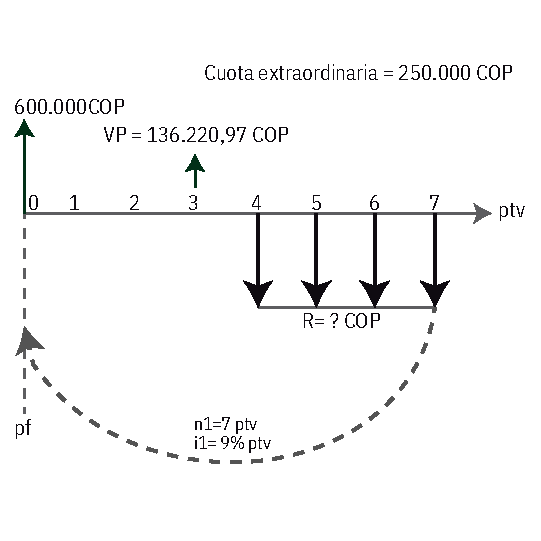
\includegraphics[trim=-78 -5 -78 -5]{7_Capitulo/img/ejemplos/2/Capitulo7Ejercicio2b.pdf} }
		
		
		\\ \hline
		%%%%%%%%%%%%% FIN INSERCIÓN DE IMAGEN
		%%%%%FIN FLUJO DE CAJA
		
		
		
		%%%%% INICIO DECLARACIÓN FORMULAS
		%%%%%%%%%%% INICIO TITULO
		\rowcolor[HTML]{FFB183}
		\multicolumn{3}{|c|}{\cellcolor[HTML]{FFB183}\textbf{4. Declaración de fórmulas}}    \\ \hline
		%%%%%%%%%%% FIN TITULO
		%%%%%%%%%%% INICIO MATEMÁTICAS
		\multicolumn{3}{|c|}{$VP=R(\frac{1-(1+i)^{-n}}{i}) \hspace{0.4 cm} \textit{Valor presente de una serie uniforme}$} \\ \hline
		
		%%%%%%%%%% FIN MATEMÁTICAS
		%%%%%% INICIO DESARROLLO MATEMÁTICO
		\rowcolor[HTML]{FFB183}
		%%%%%%%%%%INICIO TITULO
		\multicolumn{3}{|c|}{\cellcolor[HTML]{FFB183}\textbf{5. Desarrollo matemático}}       \\ \hline
		%%%%%%%%%% FIN TITULO
		%%%%%%%%%% INICIO MATEMÁTICAS
		\multicolumn{3}{|p{\textwidth}|}{Después del abono extraordinario de 250.000 COP el saldo de la deuda es ahora de 136.220,97 COP que se tomará como nuevo capital inicial, por lo tanto:} \\
		\multicolumn{3}{|c|}{$ 136{.}220 \ COP =R(\frac{1-(1+0.09)^{-4}}{0.09})\hspace{0.2 cm}\rightarrow \hspace{0.2 cm}R= 42{.}047.14 \ COP$} \\ \hline
		
		%%%%%%%%%% FIN MATEMÁTICAS
		%%%%%% FIN DESARROLLO MATEMÁTICO
		%%%%%% INICIO RESPUESTA
		\rowcolor[HTML]{FFB183}
		%%%%%%%%%%INICIO TITULO
		\multicolumn{3}{|c|}{\cellcolor[HTML]{FFB183}\textbf{6. Respuesta}}   \\ \hline
		%%%%%%%%%% FIN TITULO
		%%%%%%%%%% INICIO RESPUESTA MATEMÁTICA
		\multicolumn{3}{|c|}{$\mathbf{R = 42{.}047.14  \ COP}$}
		\begin{comment}
		\multicolumn{3}{|p{\textwidth}|}{
		$F_{4} = F_{5} = 21.609,84 COP $ .}
		\end{comment} 
		\\ \hline
		%%%%%%%%%% FIN MATEMÁTICAS
		%%%%%% FIN RESPUESTA
	\end{longtable}
	%Se crean dos lineas en blanco para que no quede el siguiente texto tan pegado
	%\newline \newline %USARLO SI CREES QUE ES NECESARIO
\end{center}
%%%%%%%%%%%%%%%%%%%%%%%%%%FIN EJERCICIO 2b %%%%%%%%%%%%%%%%%%%%%%%%%%%
Y la tabla debe ser modificada así:

\begin{spacing}{1.1}
    \footnotesize
	\begin{center}
		\begin{tabular}{|p{1cm}|p{2cm}|p{2cm}|p{2cm}|p{3cm}|}
			\hline
			\textbf{PER\ (1)} & \textbf{SALDO DEUDA (2)=(2)-(5)} & \textbf{INTERESES  (3)=(2)(i)} & \textbf{PAGO\ (4)= COP  R- COP  L } & \textbf{AMORTIZACIÓN  (5)=(4)-(3)} \\ \hline
			
			0                 &  600.000,00 \ COP                     & ---------                       & ---------                   & ---------                          \\ \hline
			1                 &  534.785,69 \ COP                     &  54.000,00 \ COP                    &  119.214,31 \ COP                &  65.214,31 \ COP                        \\ \hline
			2                 &  463.702,09 \ COP                     &  48.130,71 \ COP                    &  119.214,31 \ COP                &  71.083,60 \ COP                        \\ \hline
    3                 &  136.220,97 \ COP                     &  41.733,19 \ COP                     &  \textbf{369.214,31 \ COP }                 &  327.481,12 \ COP                       \\ \hline
			4                 &  106.433,72 \ COP                     &  12.259,89 \ COP                     &  42.047,14 \ COP                 &  29.787,25 \ COP                        \\ \hline
			5                 &  73.965,61 \ COP                      &  9.579,03 \ COP                      &  42.047,14 \ COP                 &  32.468,11 \ COP                        \\ \hline
			6                 &  38.575,37 \ COP                      &  6.656,90 \ COP                      &  42.047,14 \ COP                 &  35.390,24 \ COP                        \\ \hline
			7                 &  0,00 \ COP                           &  3.471,77 \ COP                      &  42.047,14 \ COP                 &  38.575,37 \ COP                        \\ \hline
		\end{tabular}
	\end{center}
\end{spacing}

\textbf{Observe que la cuota ordinaria baja de  119.214,31 \ COP a  42.047,14 \ COP pero se mantiene el plazo originalmente pactado}.\\
%%%%%%%%%%%%%%%%%%%%%%%%%%FIN EJERCICIO 2 %%%%%%%%%%%%%%%%%%%%%%%%%%%

\section{Amortización con periodos de gracia (*)}
El período de gracia consiste en que, después de efectuado el préstamo, va a pasar cierto tiempo antes de que se empiecen a efectuar pagos y básicamente, existen dos modalidades de préstamo con períodos de gracia:\\

\begin{itemize}
	\item\textbf{ Período de gracia muerto (*):} consiste en que, durante cierto tiempo, no hay pagos de ninguna clase, a este tiempo se le denomina "período de gracia muerto". Lógicamente, esto no se hace gratuitamente, sino que los intereses causados van acumulándose a la deuda; es decir, que durante el período de gracia muerto, la deuda incrementa. \\
	\item \textbf{Período de gracia con cuota reducida (*):} consiste en que, durante cierto tiempo se pagan unas cuotas reducidas equivalentes al valor de los intereses que se causan, pero sin hacer amortización al capital, en consecuencia, la deuda permanece constante, porque en la medida que se van causando los intereses se van pagando. Este tipo de préstamo está especialmente dirigido al sector industrial y lo denominaremos "período de gracia con cuota reducida". Obviamente, en un mismo préstamo pueden existir las dos modalidades, lo cual puede dar origen a una tercera modalidad. En este caso el período de gracia muerto siempre figurará de primero, le seguirá el período de gracia con cuota reducida y, a continuación, las cuotas ordinarias.\\
\end{itemize}

%%%%%%%%%%%%%%%%%%% EJERCICIO 3 %%%%%%
\textbf{Ejemplo 3 }\\
Se concede un préstamo de 2.000.000 COP, con un plazo de gracia muerto de 6 meses seguido de 4 cuotas trimestrales crecientes en un 10\%  y con un interés del 44\% nominal anual trimestre vencido. Elaborar la tabla de amortización.\\

%\newpage %USAR SOLO SI EL SOLUCIÓN QUEDA SOLO Y ES NECESARIO BAJARLO A LA SIGUIENTE PAGINA
\textbf{Solución.}\\
%La tabla ira centrada
\begin{center}
	\renewcommand{\arraystretch}{1.5}% Margenes de las celdas
	%Creación de la cuadricula de 3 columnas
	\begin{longtable}[H]{|c|c|c|}
		%Creamos una linea horizontal
		\hline
		%Definimos el color de la primera fila
		\rowcolor[HTML]{FFB183}
		%%%%% INICIO ASIGNACIÓN FECHA FOCAL %%%%%%%
		%%%%%%%%%% INICIO TITULO
		%Lo que se hace aquí es mezclar las 3 columnas en una sola
		\multicolumn{3}{|c|}{\cellcolor[HTML]{FFB183}\textbf{1. Asignación período focal}}  \\ \hline
		\multicolumn{3}{|c|}{$pf : \textit{0 ptv}$}   \\\hline
		%%%%%%%%%% FIN TITULO
		%%%%% INICIO DECLARACIÓN DE VARIABLES %%%%%%%
		%%%%%%%%%% INICIO TITULO
		%Lo que se hace aquí es mezclar las 3 columnas en una sola
		\multicolumn{3}{|c|}{\cellcolor[HTML]{FFB183}\textbf{2. Declaración de variables}}   \\ \hline
		%%%%%%%%%% FIN TITULO
		%%%%%%%%%% INICIO DE MATEMÁTICAS
		%Cada & hace referencia al paso de la siguiente columna
		\cellcolor[HTML]{FFB183}\textbf{Valores monetarios} & 
		\cellcolor[HTML]{FFB183}\textbf{Valores no monetarios} & 
		\cellcolor[HTML]{FFB183}\textbf{Incógnitas}  \\ \hline
	 	$ \hspace{1cm} VP= 2{.}000{.}000 \ COP \hspace{1cm}$ & $\hspace{1.5cm} i = 11\% \textit{ ptv} \hspace{1.5cm}$ & $ R=\textit{?COP} $ \\
		& $ n=4 \textit{ ptv} $ &  \\
		& $ j=44\% \textit{ natv} $ &  \\
		& $ g=10\% $ &  \\ \hline
		
		
		%%%%%%%%%% FIN DE MATEMÁTICAS
		%%%%% FIN DECLARACIÓN DE VARIABLES
		
		
		%%%%% INICIO FLUJO DE CAJA
		\rowcolor[HTML]{FFB183}
		\multicolumn{3}{|c|}{\cellcolor[HTML]{FFB183}\textbf{3. Diagrama de flujo de caja}} \\ \hline
		%Mezclamos 3 columnas y pondremos el dibujo
		%%%%%%%%%%%%% INSERCIÓN DE LA IMAGEN
		%Deberán descargar las imágenes respectivas del drive y pegarlas en la carpeta
		%n_capitulo/img/ejemplos/1/capitulo1ejemplo1.pdf  (el /1/ es el numero del ejemplo)
		\multicolumn{3}{|c|}{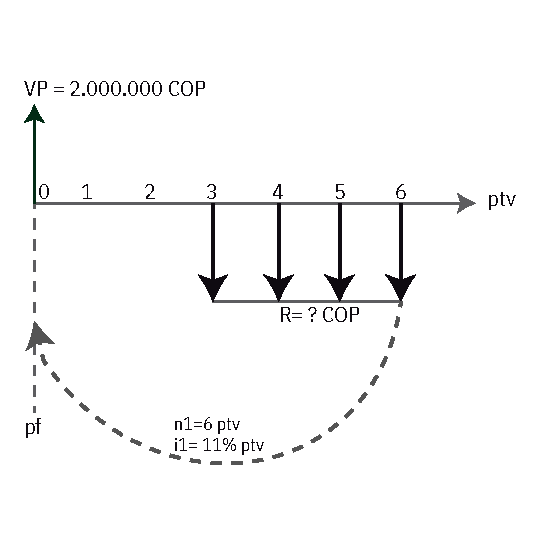
\includegraphics[trim=-78 -5 -78 -5]{7_Capitulo/img/ejemplos/3/Capitulo7Ejercicio3.pdf} }
		
		
		\\ \hline
		%%%%%%%%%%%%% FIN INSERCIÓN DE IMAGEN
		%%%%%FIN FLUJO DE CAJA
		
		
		
		%%%%% INICIO DECLARACIÓN FORMULAS
		%%%%%%%%%%% INICIO TITULO
		\rowcolor[HTML]{FFB183}
		\multicolumn{3}{|c|}{\cellcolor[HTML]{FFB183}\textbf{4. Declaración de fórmulas}}    \\ \hline
		%%%%%%%%%%% FIN TITULO
		%%%%%%%%%%% INICIO MATEMÁTICAS
        \multicolumn{3}{|c|}{$F=P(1+i)^{n} \hspace{0.4 cm} \textit{Valor futuro}$} \\
        \multicolumn{3}{|c|}{$VP=R(\frac{R(1+g)^{n}(1+i)^{n}-1}{g-i})$   \hspace{0.4 cm}\textit{Valor presente de gradiente geométrico, si $g \neq i$} } \\ \hline
		
		%%%%%%%%%% FIN MATEMÁTICAS
		%%%%%% INICIO DESARROLLO MATEMÁTICO
		\rowcolor[HTML]{FFB183}
		%%%%%%%%%%INICIO TITULO
		\multicolumn{3}{|c|}{\cellcolor[HTML]{FFB183}\textbf{5. Desarrollo matemático}}       \\ \hline
		%%%%%%%%%% FIN TITULO
		%%%%%%%%%% INICIO MATEMÁTICAS
		\multicolumn{3}{|c|}{$  2{.}000{.}000 \ COP = R(\frac{[(1+0.1)^{4}(1+0.11)^{-4}-1]}{0.1-0.11})(1+0.11)^{-2}\hspace{0.2 cm}\rightarrow \hspace{0.2 cm}R= 693{.}125.94 \ COP$} \\ \hline
		
		%%%%%%%%%% FIN MATEMÁTICAS
		%%%%%% FIN DESARROLLO MATEMÁTICO
		%%%%%% INICIO RESPUESTA
		\rowcolor[HTML]{FFB183}
		%%%%%%%%%%INICIO TITULO
		\multicolumn{3}{|c|}{\cellcolor[HTML]{FFB183}\textbf{6. Respuesta}}   \\ \hline
		%%%%%%%%%% FIN TITULO
		%%%%%%%%%% INICIO RESPUESTA MATEMÁTICA
		\multicolumn{3}{|c|}{$\mathbf{R= 693{.}125.94 \ COP}$}
		\begin{comment}
		\multicolumn{3}{|p{\textwidth}|}{
		$F_{4} = F_{5} = 21.609,84 \ COP $ .}
		\end{comment} 
		\\ \hline
		%%%%%%%%%% FIN MATEMÁTICAS
		%%%%%% FIN RESPUESTA
	\end{longtable}
	%Se crean dos lineas en blanco para que no quede el siguiente texto tan pegado
	%\newline \newline %USARLO SI CREES QUE ES NECESARIO
\end{center}
%%%%%%%%%%%%%%%%%%%%%%%%%%FIN EJERCICIO 3 %%%%%%%%%%%%%%%%%%%%%%%%%%%


La Tabla de Amortización correspondiente es:
\begin{spacing}{1.1}
	\begin{center}
    \footnotesize
		\begin{tabular}{|p{1cm}|p{2.5cm}|p{2.5cm}|p{2.5cm}|p{3cm}|}
			\hline
			\rowcolor{white!50}
			\textbf{PER\ (1)} & \textbf{SALDO DEUDA (2)=(2)-(5)} & \textbf{INTERESES  (3)=(2)(i)} & \textbf{PAGO\ (4)= R COP - L COP} & \textbf{AMORTIZACIÓN  (5)=(4)-(3)} \\ \hline
			
			0                 &  2.000.000,00 \ COP                  & ---------                       & ---------                   & ---------                          \\ \hline
			1                 &  2.000.000,00 \ COP                   &  220.000,00 \ COP                   & 0,00 \ COP                      &  -220.000,00 \ COP                      \\ \hline
			2                 &  2.464.200,00 \ COP                   &  244.200,00 \ COP                   &  0,00 \ COP                      &  -244.200,00 \ COP                      \\ \hline
			3                 &  2.042.236,06 \ COP                   &  271.062,00 \ COP                    &  693.125,94 \ COP                &  422.063,94 \ COP                       \\ \hline
			4                 &  1.504.332,50 \ COP                   &  224.634,97 \ COP                    &  762.438,53 \ COP                &  537.803,56 \ COP                       \\ \hline
			5                 &  831.126,69 \ COP                     &  165.476,58 \ COP                    &  838.682,39 \ COP                &  673.205,81 \ COP                       \\ \hline
			6                 &  0,00 \ COP                           &  91.423,94 \ COP                     &  922.550,63 \ COP                &  831.126,69 \ COP                       \\ \hline
		\end{tabular}
	\end{center}
\end{spacing}

\textbf{Observación: } La amortización de los períodos 1 y 2 es negativa; esto significa que hay una desamortización o aumento de deuda.\\

%%%%%%%%%%%%%%%%%%% EJERCICIO 4 %%%%%%
\textbf{Ejemplo 4}\\
Elaborar una tabla para amortizar la suma de  2.000.000 COP , en las siguientes condiciones:\\
a)	plazo de gracia muerto 6 meses\\
b)	plazo de gracia con cuota reducida al pago de los intereses \\
c)	4 cuotas uniformes a partir del período 4\\
d)	cuota extraordinaria pactada  150.000 COP, en el período 7\\
e)	tasa de interés del 21\% nominal anual trimestre vencido\\


%%%%%%%%%%%%%%%%%%% EJERCICIO 4a-d %%%%%%

%\newpage %USAR SOLO SI EL SOLUCIÓN QUEDA SOLO Y ES NECESARIO BAJARLO A LA SIGUIENTE PAGINA
\textbf{Solución.\\ a), b), c), d)}\\
%La tabla ira centrada
\begin{center}
	\renewcommand{\arraystretch}{1.5}% Margenes de las celdas
	%Creación de la cuadricula de 3 columnas
	\begin{longtable}[H]{|c|c|c|}
		%Creamos una linea horizontal
		\hline
		%Definimos el color de la primera fila
		\rowcolor[HTML]{FFB183}
		%%%%% INICIO ASIGNACIÓN PERIODO FOCAL %%%%%%%
		%%%%%%%%%% INICIO TITULO
		%Lo que se hace aquí es mezclar las 3 columnas en una sola
		\multicolumn{3}{|c|}{\cellcolor[HTML]{FFB183}\textbf{1. Asignación período focal}}  \\ \hline
		\multicolumn{3}{|c|}{$pf : \textit{0 ptv}$}   \\\hline
		%%%%%%%%%% FIN TITULO
		%%%%% INICIO DECLARACIÓN DE VARIABLES %%%%%%%
		%%%%%%%%%% INICIO TITULO
		%Lo que se hace aquí es mezclar las 3 columnas en una sola
		\multicolumn{3}{|c|}{\cellcolor[HTML]{FFB183}\textbf{2. Declaración de variables}}   \\ \hline
		%%%%%%%%%% FIN TITULO
		%%%%%%%%%% INICIO DE MATEMÁTICAS
		%Cada & hace referencia al paso de la siguiente columna
		\cellcolor[HTML]{FFB183}\textbf{Valores monetarios} & 
		\cellcolor[HTML]{FFB183}\textbf{Valores no monetarios} & 
		\cellcolor[HTML]{FFB183}\textbf{Incógnitas}  \\ \hline
	 	$ \hspace{1cm} VP= 2{.}000{.}000 \ COP \hspace{1cm}$ & $\hspace{1.5cm} i = 5.25\% \textit{ ptv} \hspace{1.5cm}$ & $ R=\textit{?COP} $ \\
		$ \hspace{1cm} F_2= 150{.}000 \ COP \hspace{1cm}$ & $ n_0=2 \textit{ ptv} $ &  \\
		& $ n_1=4 \textit{ ptv} $ &  \\
		& $ n_2=7 \textit{ ptv} $ &  \\
		& $ j = 21\% \textit{ natv} $ &  \\ \hline
		
		
		
		%%%%%%%%%% FIN DE MATEMÁTICAS
		%%%%% FIN DECLARACIÓN DE VARIABLES
		
		
		%%%%% INICIO FLUJO DE CAJA
		\rowcolor[HTML]{FFB183}
		\multicolumn{3}{|c|}{\cellcolor[HTML]{FFB183}\textbf{3. Diagrama de flujo de caja}} \\ \hline
		%Mezclamos 3 columnas y pondremos el dibujo
		%%%%%%%%%%%%% INSERCIÓN DE LA IMAGEN
		%Deberán descargar las imágenes respectivas del drive y pegarlas en la carpeta
		%n_capitulo/img/ejemplos/1/capitulo1ejemplo1.pdf  (el /1/ es el numero del ejemplo)
		\multicolumn{3}{|c|}{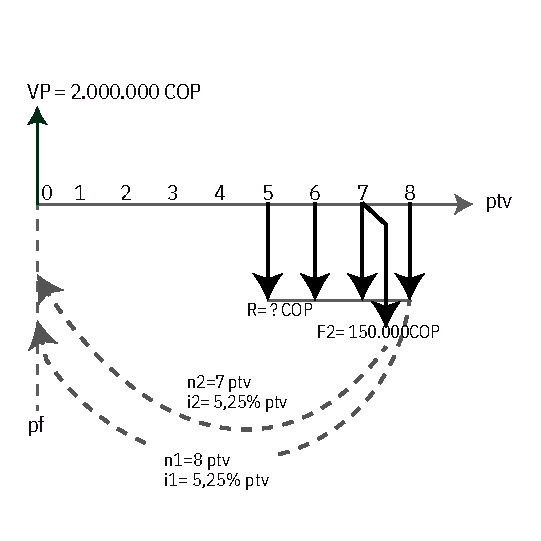
\includegraphics[trim=-78 -5 -78 -5]{7_Capitulo/img/ejemplos/4/Capitulo7Ejercicio4.pdf} }
		
		
		\\ \hline
		%%%%%%%%%%%%% FIN INSERCIÓN DE IMAGEN
		%%%%%FIN FLUJO DE CAJA
		
		
		
		%%%%% INICIO DECLARACIÓN FORMULAS
		%%%%%%%%%%% INICIO TITULO
		\rowcolor[HTML]{FFB183}
		\multicolumn{3}{|c|}{\cellcolor[HTML]{FFB183}\textbf{4. Declaración de fórmulas}}    \\ \hline
		%%%%%%%%%%% FIN TITULO
		%%%%%%%%%%% INICIO MATEMÁTICAS
		\multicolumn{3}{|c|}{$F=P(1+i)^{n} \hspace{0.4 cm} \textit{Valor futuro}$} \\
		\multicolumn{3}{|c|}{$VP=R(\frac{1-(1+i)^{-n}}{i}) \hspace{0.4 cm} \textit{Valor presente de una serie uniforme vencida}$} \\ \hline
		
		%%%%%%%%%% FIN MATEMÁTICAS
		%%%%%% INICIO DESARROLLO MATEMÁTICO
		\rowcolor[HTML]{FFB183}
		%%%%%%%%%%INICIO TITULO
		\multicolumn{3}{|c|}{\cellcolor[HTML]{FFB183}\textbf{5. Desarrollo matemático}}       \\ \hline
		%%%%%%%%%% FIN TITULO
		%%%%%%%%%% INICIO MATEMÁTICAS
		\multicolumn{3}{|p{\textwidth}|}{Los períodos 1 y 2 son de gracia muertos; los períodos 3 y 4 son de gracia con cuota reducida al valor de los intereses sobre la deuda, capitalizados los intereses en el período de gracias: los periodos 5 al 8 son de cuota ordinaria; en el período 2 la deuda sera: } \\
		\multicolumn{3}{|c|}{$F= 2{.}000{.}000 \ COP (1+0.0525)^{2}= 2{.}215{.}512.50 \ COP $} \\ 
		\multicolumn{3}{|p{\textwidth}|}{El valor del interés I de los períodos 3 y 4, se calcula aplicando la tasa a la deuda que hay en el período 2: } \\ 
		\multicolumn{3}{|c|}{$( 2{.}215{.}512.50 \ COP)(0.0525)= 116{.}314.41 \ COP$} \\
		\multicolumn{3}{|p{\textwidth}|}{La ecuación de valor quedará así: } \\ 
		\multicolumn{3}{|c|}{$ 2{.}000{.}000 \ COP =  116{.}314.41 \ COP (\frac{1-(1+0.0525)^{-2}}{0,0525})(1+0.05251)^{-2}+ $} \\
		\multicolumn{3}{|c|}{$+R(\frac{1-(1+0.0525)^{-4}}{0,0525})(1+0.05251)^{-4}+  150{.}000 \ COP (1,0525)^{-7}\hspace{0.4 cm} $} \\\hline
		%%%%%%%%%% FIN MATEMÁTICAS
		%%%%%% FIN DESARROLLO MATEMÁTICO
		%%%%%% INICIO RESPUESTA
		\rowcolor[HTML]{FFB183}
		%%%%%%%%%%INICIO TITULO
		\multicolumn{3}{|c|}{\cellcolor[HTML]{FFB183}\textbf{6. Respuesta}}   \\ \hline
		%%%%%%%%%% FIN TITULO
		%%%%%%%%%% INICIO RESPUESTA MATEMÁTICA
		\multicolumn{3}{|c|}{$\mathbf{R= 591{.}940.10 \ COP}$}
		\begin{comment}
		\multicolumn{3}{|p{\textwidth}|}{
		$F_{4} = F_{5} = 21.609,84 \ COP $ .}
		\end{comment} 
		\\ \hline
		%%%%%%%%%% FIN MATEMÁTICAS
		%%%%%% FIN RESPUESTA
	\end{longtable}
	%Se crean dos lineas en blanco para que no quede el siguiente texto tan pegado
	%\newline \newline %USARLO SI CREES QUE ES NECESARIO
\end{center}
%%%%%%%%%%%%%%%%%%% FIN EJERCICIO 4a-d %%%%%%
%%%%%%%%%%%%%%%%%%% EJERCICIO 4e %%%%%%
\textbf{Respuesta.\\e)\\}
	La tabla de Amortización será: \\
	\begin{spacing}{1.1}
		\begin{center}
        \footnotesize
			\begin{tabular}{|p{1cm}|p{2.5cm}|p{2.5cm}|p{2cm}|p{3cm}|}
				\hline
				\textbf{PER\ (1)} & \textbf{SALDO DEUDA (2)=(2)-(5)} & \textbf{INTERESES  (3)=(2)(i)} & \textbf{PAGO\ (4)=R  COP  -  L  COP} & \textbf{AMORTIZACIÓN  (5)=(4)-(3)} \\ \hline
				
				0                 &  2.000.000 COP                      & ---------                       & ---------                       & ---------                          \\ \hline
				1                 &  2.105.000  COP                      &  105.000  COP                   &  0,00  COP                    &    -105.000  COP                    \\ \hline
				2                 &  2.215.512  COP                      &  110.512  COP                   &  0,00  COP                    &    -110.512  COP                   \\ \hline
				3                 &  2.215.512  COP                      &  116.314  COP                  &  116.314  COP                  &    0,00  COP                           \\ \hline
				4                 &  2.215.512  COP                      &  116.314  COP                  &  116.314  COP                  &    0,00  COP                           \\ \hline
				5                 &  1.739.886  COP                       &  116.314  COP                  &  591.940  COP                 &    475.625,59   COP                    \\ \hline
				6                 &  1.239.290  COP                       &  91.344  COP                   &  591.940  COP                 &    500.596  COP                     \\ \hline
				7                 &  562.413  COP                        &   65.062  COP                   &  741.940  COP                 &    676.877   COP                   \\ \hline
				8                 &  0,00  COP                           &  29.526  COP                &    591.940  COP                   &    562.413   COP                    \\ \hline
			\end{tabular}
		\end{center}
	\end{spacing}
	\textbf{Observaciones: }\\
	1)	La amortización de los períodos 1 y 2 es negativa; esto significa que hay una desamortización o aumento de deuda.\\
	2)	La amortización de los períodos 3 y 4 es cero, debido a que se pagan los intereses.\\
	3)	 El valor del pago en el período 7 es igual a la suma del pago ordinario, más el pago extraordinario, por tanto:  591.940,1 
 COP  +  150.000  COP  =  741.940,1  COP.\\
%%%%%%%%%%%%%%%%%%%%%%%%%%FIN EJERCICIO 4e %%%%%%%%%%%%%%%%%%%%%%%%%%%
%%%%%%%%%%%%%%%%%%%%%%%%%%FIN EJERCICIO 4 %%%%%%%%%%%%%%%%%%%%%%%%%%%
	
	\section{Distribución de un pago}
	
	Cada cuota de amortización está compuesta de dos partes: la que corresponde a intereses y la que corresponde a amortización; sin embargo, no es necesario construir la tabla para establecer la proporción en que una cuota dada se divide entre interés y amortización. Basta con calcularle los intereses al capital insoluto del período inmediatamente anterior y luego, restárselo al valor de la cuota, para conocer la parte que corresponde a la amortización. \\
	
	%%%%%%%%%%%%%%%%%%%%%%%%%%EJERCICIO 5 %%%%%%%%%%%%%%%%%%%%%%%%%%%

\textbf{Ejemplo 5}\\
Hallar la distribución del pago número 125 periodo mes vencido (valor de los intereses y del capital amortizado), en una amortización de  2.000.000 COP, mediante pagos mensuales durante 20 años, suponiendo una tasa del 30\% nominal anual mes vencido.

%\newpage %USAR SOLO SI EL SOLUCIÓN QUEDA SOLO Y ES NECESARIO BAJARLO A LA SIGUIENTE PAGINA

\textbf{Solución 5.}\\
%La tabla ira centrada
\begin{center}
	\renewcommand{\arraystretch}{1.5}% Margenes de las celdas
	%Creación de la cuadricula de 3 columnas
	\begin{longtable}[H]{|c|c|c|}
		%Creamos una linea horizontal
		\hline
		%Definimos el color de la primera fila
		\rowcolor[HTML]{FFB183}
		%%%%% INICIO ASIGNACIÓN PERIODO FOCAL %%%%%%%
		%%%%%%%%%% INICIO TITULO
		%Lo que se hace aquí es mezclar las 3 columnas en una sola
		\multicolumn{3}{|c|}{\cellcolor[HTML]{FFB183}\textbf{1. Asignación período focal}}   \\ \hline
		%%%%%%%%%% FIN TITULO
		%%%%% INICIO DECLARACIÓN DE VARIABLES %%%%%%%
		\multicolumn{3}{|c|}{$pf : 0 \textit{ ptv}$}\\ \hline
		%%%%%%%%%% INICIO TITULO
		%Lo que se hace aquí es mezclar las 3 columnas en una sola
		\multicolumn{3}{|c|}{\cellcolor[HTML]{FFB183}\textbf{2. Declaración de variables}}   \\ \hline
		%%%%%%%%%% FIN TITULO
		%%%%%%%%%% INICIO DE MATEMÁTICAS
		%Cada & hace referencia al paso de la siguiente columna
		\cellcolor[HTML]{FFB183}\textbf{Valores monetarios} & 
		\cellcolor[HTML]{FFB183}\textbf{Valores no monetarios} & 
		\cellcolor[HTML]{FFB183}\textbf{Incógnitas}  \\ \hline
		$ \hspace{1cm} VP= 2{.}000{.}000 \ COP \hspace{1cm}$ & $\hspace{1.5cm} i =  2.5\% \textit{ pmv} \hspace{1.5cm}$ & $ R=\textit{?COP} $ \\
		& $ n = 125 \textit{ pmv} $ & $ I=\textit{?COP} $ \\
		& $ j = 30\% \textit{ namv} $ & $ A=\textit{?COP} $ \\ \hline

		%%%%%%%%%% FIN DE MATEMÁTICAS
		%%%%% FIN DECLARACIÓN DE VARIABLES
		
		\rowcolor[HTML]{FFB183}
		\multicolumn{3}{|c|}{\cellcolor[HTML]{FFB183}\textbf{3. Diagrama de flujo de caja}} \\ \hline
		\multicolumn{3}{|c|}{ 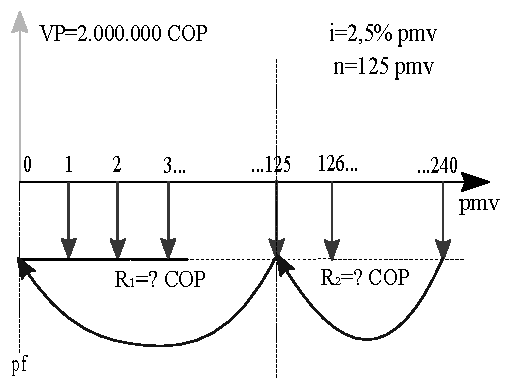
\includegraphics[trim=-78 -5 -78 -5]{7_Capitulo/img/ejemplos/5/5_1.pdf} }   \\ \hline
		%%%%% INICIO FLUJO DE CAJA
		\rowcolor[HTML]{FFB183}
		\multicolumn{3}{|c|}{\cellcolor[HTML]{FFB183}\textbf{4. Declaración de fórmulas}} \\ \hline
		%%%%%%%%%%%%% FIN INSERCIÓN DE IMAGEN
		%%%%%FIN FLUJO DE CAJA
		
		\multicolumn{3}{|c|}{ $VP = R \frac{1-(1+i)^{-n}}{i} $ Valor presente serie uniforme vencido }   \\ 
		\multicolumn{3}{|c|}{ $I = P \hspace{1mm} i $ Interés periódico }   \\ 
		\multicolumn{3}{|c|}{ $A = R - I $ Amortización a capital, una vez descontados los intereses de la cuota R }   \\ \hline
		
		%%%%%% INICIO DESARROLLO MATEMÁTICO
		\rowcolor[HTML]{FFB183}
		%%%%%%%%%%INICIO TITULO
		\multicolumn{3}{|c|}{\cellcolor[HTML]{FFB183}\textbf{5. Desarrollo matemático}}       \\ \hline
		%%%%%%%%%% FIN TITULO
		%%%%%%%%%% INICIO MATEMÁTICAS
		\multicolumn{3}{|C{\linewidth}|}{
			Como todos los pagos son iguales, entonces el valor del pago 125 se obtiene de la siguiente ecuación:
			
		
			$  2$.$000$.$000 \hspace{1mm} COP  = R \frac{1-(1+ 0,025)^{-240}}{0,025} $ Ecuación de valor
		
				$Donde \hspace{1mm} R =  5$.$133,78 \hspace{1mm} COP$
		
			Por otra parte se sabe que la porción de la cuota 125 pmv que se utiliza para pagar intereses es igual a la tasa, multiplicada por la deuda que queda inmediatamente después de haberse efectuado el pago número 124 pmv. Entonces, para hallar la deuda, en ese momento, debemos calcular el valor presente de los pagos que faltan por hacer.
			
			Como en total hay 240 pagos y se han hecho 124 entonces faltan por hacer 116 pagos. El valor presente de estos pagos en el punto 124 será:
			
			$ VP =   5$.$133,78 \hspace{1mm} COP  \frac{1-(1+ 0,025)^{-116}}{0,025} =   1$.$891$.$004,92 \hspace{1mm}  COP\hspace{1mm} deuda \hspace{1mm}en\hspace{1mm} la \hspace{1mm}cuota \hspace{1mm}124 $ 
			
			Y los intereses serán:
			
			$ I= (  1$.$891$.$004,92 \hspace{1mm} COP)(0,025) =  47$.$275,12 \hspace{1mm} COP$
			
			Finalmente, la amortización será igual a la cuota menos intereses
			
			$ A= (  5$.$133,78 \hspace{1mm} COP)-( 47$.$275,12 \hspace{1mm} COP) =   2$.$858,66 \hspace{1mm} COP$
			
		}\\ \hline
		
		%%%%%%%%%% FIN MATEMÁTICAS
		%%%%%% FIN DESARROLLO MATEMÁTICO
		%%%%%% INICIO RESPUESTA
		\rowcolor[HTML]{FFB183}
		%%%%%%%%%%INICIO TITULO
		\multicolumn{3}{|c|}{\cellcolor[HTML]{FFB183}\textbf{6. Respuesta}}   \\ \hline
		%%%%%%%%%% FIN TITULO
		%%%%%%%%%% INICIO RESPUESTA MATEMÁTICA
		\multicolumn{3}{|c|}{ 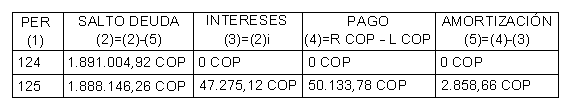
\includegraphics[trim=-78 -5 -78 -5]{7_Capitulo/img/ejemplos/5/5_2.pdf} }   \\ \hline			
		%%%%%%%%%% FIN MATEMÁTICAS
		%%%%%% FIN RESPUESTA
	\end{longtable}
	%Se crean dos lineas en blanco para que no quede el siguiente texto tan pegado
	%\newline \newline %USARLO SI CREES QUE ES NECESARIO
\end{center}
%%%%%%%%%%%%%%%%%%%%%%%%%%FIN EJERCICIO 5 %%%%%%%%%%%%%%%%%%%%%%%%%%%
 
	%%%%%%%%%%%%%%%%%%%%%%%%%%EJERCICIO 6 %%%%%%%%%%%%%%%%%%%%%%%%%%%
%%%%%%%%%%%%%%%%%%%%%%%%%%EJERCICIO 6a %%%%%%%%%%%%%%%%%%%%%%%%%%%

\textbf{Ejemplo 6}\\
Hallar la distribución del pago 58 en una amortización de 5.000.000 COP en pagos mensuales durante 10 años. Suponga que los pagos son crecientes en un 2\% y que la tasa es del 3\% periódico mes vencido.

%\newpage %USAR SOLO SI EL SOLUCIÓN QUEDA SOLO Y ES NECESARIO BAJARLO A LA SIGUIENTE PAGINA

\textbf{Solución 6.}\\
%La tabla ira centrada
\begin{center}
	\renewcommand{\arraystretch}{1.5}% Margenes de las celdas
	%Creación de la cuadricula de 3 columnas
	\begin{longtable}[H]{|c|c|c|}
		%Creamos una linea horizontal
		\hline
		%Definimos el color de la primera fila
		\rowcolor[HTML]{FFB183}
		%%%%% INICIO ASIGNACIÓN PERIODO FOCAL %%%%%%%
		%%%%%%%%%% INICIO TITULO
		%Lo que se hace aquí es mezclar las 3 columnas en una sola
		\multicolumn{3}{|c|}{\cellcolor[HTML]{FFB183}\textbf{1. Asignación período focal}}   \\ \hline
		%%%%%%%%%% FIN TITULO
		%%%%% INICIO DECLARACIÓN DE VARIABLES %%%%%%%
		\multicolumn{3}{|c|}{$pf : 0 \textit{ pmv}$}\\ \hline
		%%%%%%%%%% INICIO TITULO
		%Lo que se hace aquí es mezclar las 3 columnas en una sola
		\multicolumn{3}{|c|}{\cellcolor[HTML]{FFB183}\textbf{2. Declaración de variables}}   \\ \hline
		%%%%%%%%%% FIN TITULO
		%%%%%%%%%% INICIO DE MATEMÁTICAS
		%Cada & hace referencia al paso de la siguiente columna
		\cellcolor[HTML]{FFB183}\textbf{Valores monetarios} & 
		\cellcolor[HTML]{FFB183}\textbf{Valores no monetarios} & 
		\cellcolor[HTML]{FFB183}\textbf{Incógnitas}  \\ \hline
	 	$ \hspace{1cm} VP= 5$.$000$.$000 \ COP \hspace{1cm}$ & $\hspace{1.5cm} i = 3\% \textit{ pmv} \hspace{1.5cm}$ & $ R_1=\textit{?COP} $ \\
		& $ n = 120 \textit{ pmv} $ &  \\
		& $ g = 2\% $ &  \\ \hline
		%%%%%%%%%% FIN DE MATEMÁTICAS
		%%%%% FIN DECLARACIÓN DE VARIABLES
		
		\rowcolor[HTML]{FFB183}
		\multicolumn{3}{|c|}{\cellcolor[HTML]{FFB183}\textbf{3. Diagrama de flujo de caja}} \\ \hline
		\multicolumn{3}{|c|}{ 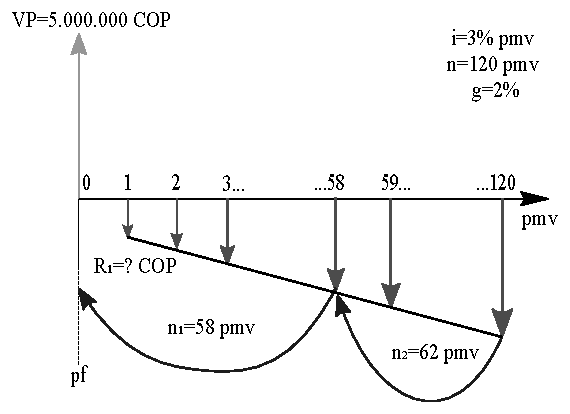
\includegraphics[trim=-78 -5 -78 -5]{7_Capitulo/img/ejemplos/6/6_1.pdf} }   \\ \hline
		%%%%% INICIO FLUJO DE CAJA
		\rowcolor[HTML]{FFB183}
		\multicolumn{3}{|c|}{\cellcolor[HTML]{FFB183}\textbf{4. Declaración de fórmulas}} \\ \hline
		%%%%%%%%%%%%% FIN INSERCIÓN DE IMAGEN
		%%%%%FIN FLUJO DE CAJA
		
		\multicolumn{3}{|c|}{ $VP = \frac{R(1+g)^{n} (1+i)^{n}-1}{g-i} $ Valor presente de un gradiente geométrico si g$ \neq $i }   \\ 
		\multicolumn{3}{|c|}{ $I = P \hspace{1mm} i $ Interés periódico }   \\ 
		\multicolumn{3}{|c|}{ $A = R - I $ Amortización a capital, una vez descontados los intereses de la cuota R }   \\ 
		\multicolumn{3}{|c|}{ $R_{n} = R_{1}(1 + g)^{n-1} $ Valor flujo de un gradiente aritmético }   \\ \hline
		
		%%%%%% INICIO DESARROLLO MATEMÁTICO
		\rowcolor[HTML]{FFB183}
		%%%%%%%%%%INICIO TITULO
		\multicolumn{3}{|c|}{\cellcolor[HTML]{FFB183}\textbf{5. Desarrollo matemático}}       \\ \hline
		%%%%%%%%%% FIN TITULO
		%%%%%%%%%% INICIO MATEMÁTICAS
		\multicolumn{3}{|C{\linewidth}|}{
			Lo primero es calcular R1 con el fin de poder hallar el valor de R58 y saber qué es lo que va a repartir.
			
			
				$  5$.$000$.$000 \hspace{1mm} COP  = \frac{ R(1+ 0,02)^{120} (1+ 0,03)^{120}-1}{0,02- 0,03} $
			
			$R_{1} =  72$.$478,16 \hspace{1mm} COP$
			
			
		}\\ \hline
		
		%%%%%%%%%% FIN MATEMÁTICAS
		%%%%%% FIN DESARROLLO MATEMÁTICO
		%%%%%% INICIO RESPUESTA
		\rowcolor[HTML]{FFB183}
		%%%%%%%%%%INICIO TITULO
		\multicolumn{3}{|c|}{\cellcolor[HTML]{FFB183}\textbf{6. Respuesta}}   \\ \hline
		%%%%%%%%%% FIN TITULO
		%%%%%%%%%% INICIO RESPUESTA MATEMÁTICA
		%\multicolumn{3}{|c|}{ 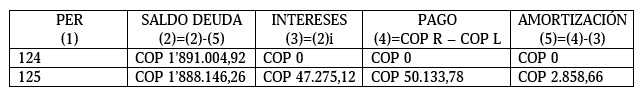
\includegraphics[trim=-78 -5 -78 -5]{7_Capitulo/img/ejemplos/5/5_2.jpg} }   \\ \hline
		\multicolumn{3}{|C{\textwidth}|}{
			$R_{58} =  72$.$478,16 \hspace{1mm} COP(1 + 0,02)^{57} =  224$.$087,15 \hspace{1mm} COP$ 
		}  \\ \hline
		
		
		%%%%%%%%%% FIN MATEMÁTICAS
		%%%%%% FIN RESPUESTA
	\end{longtable}
	%Se crean dos lineas en blanco para que no quede el siguiente texto tan pegado
	%\newline \newline %USARLO SI CREES QUE ES NECESARIO
\end{center}
%%%%%%%%%%%%%%%%%%%%%%%%%%FIN EJERCICIO 6a %%%%%%%%%%%%%%%%%%%%%%%%%%%
%%%%%%%%%%%%%%%%%%%%%%%%%%EJERCICIO 6B %%%%%%%%%%%%%%%%%%%%%%%%%%%
Para saber qué tanto del pago 58 se destina a intereses, es necesario conocer la deuda en el punto 57 y este valor se multiplica por la tasa de interés.\\

Entonces la deuda en el punto 57 será igual al valor presente en ese punto de lo que falta por pagar, pero lo que falta por pagar es un gradiente geométrico de 63 períodos (120 - 57 = 63) cuyo primer pago es de 224.087,15  COP, por lo tanto, la deuda en el período 57 será:\\

%La tabla ira centrada
\begin{center}
	\renewcommand{\arraystretch}{1.5}% Margenes de las celdas
	%Creación de la cuadricula de 3 columnas
	\begin{longtable}[H]{|c|c|c|}
		%Creamos una linea horizontal
		\hline
		%Definimos el color de la primera fila
		\rowcolor[HTML]{FFB183}
		%%%%% INICIO ASIGNACIÓN PERIODO FOCAL %%%%%%%
		%%%%%%%%%% INICIO TITULO
		%Lo que se hace aquí es mezclar las 3 columnas en una sola
		\multicolumn{3}{|c|}{\cellcolor[HTML]{FFB183}\textbf{1. Asignación período focal}}   \\ \hline
		%%%%%%%%%% FIN TITULO
		%%%%% INICIO DECLARACIÓN DE VARIABLES %%%%%%%
		\multicolumn{3}{|c|}{$pf : 0 \textit{ pmv}$}\\ \hline
		%%%%%%%%%% INICIO TITULO
		%Lo que se hace aquí es mezclar las 3 columnas en una sola
		\multicolumn{3}{|c|}{\cellcolor[HTML]{FFB183}\textbf{2. Declaración de variables}}   \\ \hline
		%%%%%%%%%% FIN TITULO
		%%%%%%%%%% INICIO DE MATEMÁTICAS
		%Cada & hace referencia al paso de la siguiente columna
		\cellcolor[HTML]{FFB183}\textbf{Valores monetarios} & 
		\cellcolor[HTML]{FFB183}\textbf{Valores no monetarios} & 
		\cellcolor[HTML]{FFB183}\textbf{Incógnitas}  \\ \hline
	 	$ \hspace{1cm} VP= 5$.$000$.$000 \ COP \hspace{1cm}$ & $\hspace{1.5cm} i = 3\% \textit{ pmv} \hspace{1.5cm}$ & $ R_1=\textit{?COP} $ \\
		& $ n = 63 \textit{ p(dias)v} = 2.1 \textit{ pmv} $ & $D = ?$ \\
		& $ g = 2\% $ &  \\ \hline
		%%%%%%%%%% FIN DE MATEMÁTICAS
		%%%%% FIN DECLARACIÓN DE VARIABLES
		
		\rowcolor[HTML]{FFB183}
		\multicolumn{3}{|c|}{\cellcolor[HTML]{FFB183}\textbf{3. Diagrama de flujo de caja}} \\ \hline
		\multicolumn{3}{|c|}{ 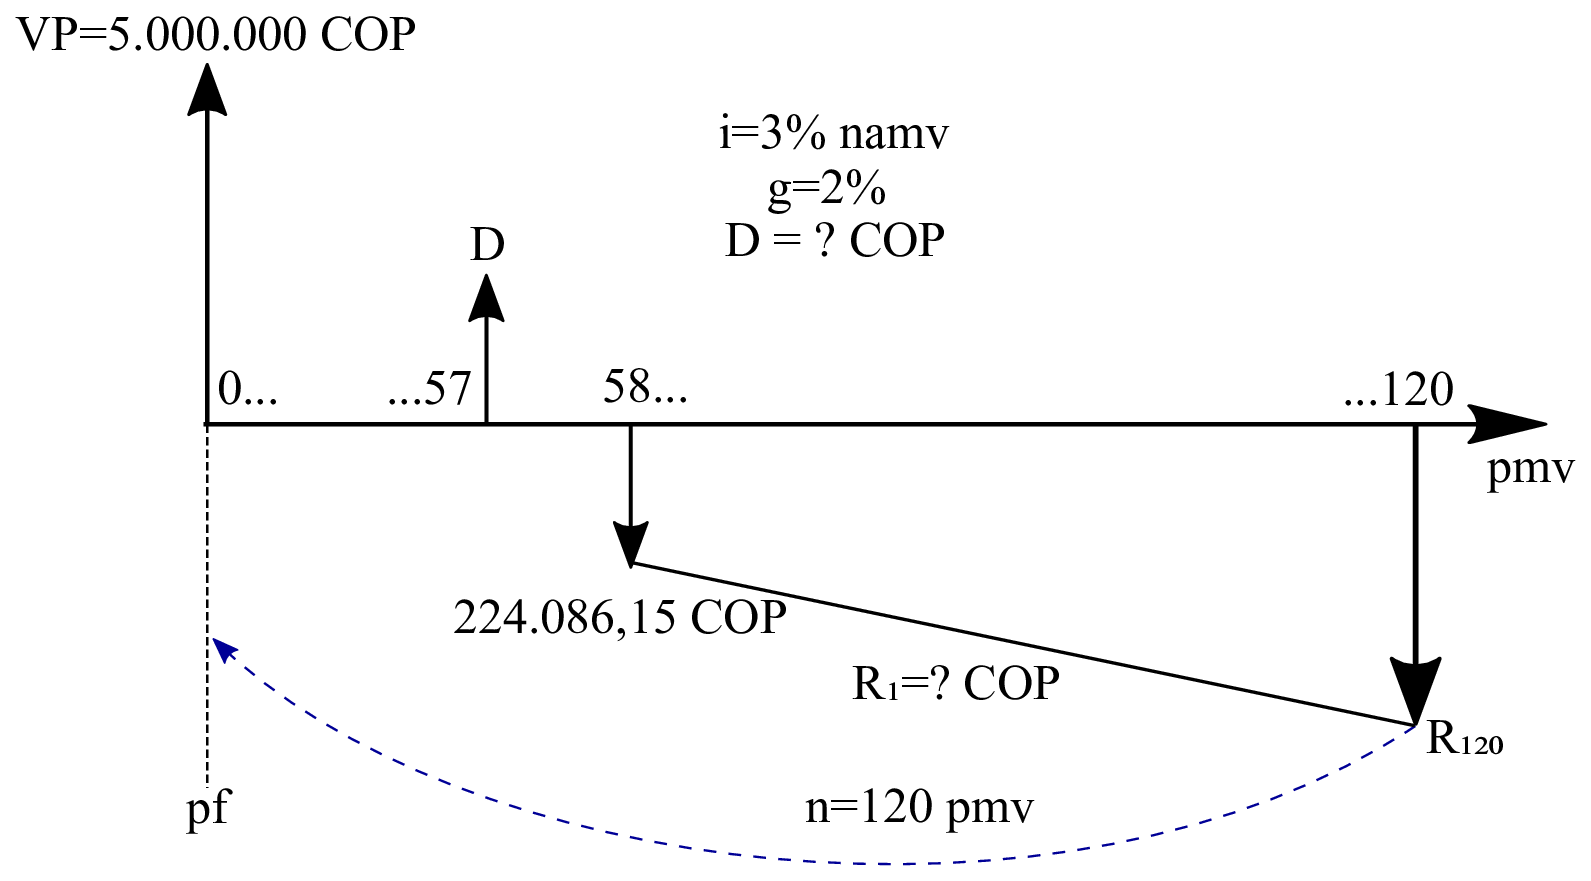
\includegraphics[scale=0.20]{7_Capitulo/img/ejemplos/6/6_2.png} }   \\ \hline
		%%%%% INICIO FLUJO DE CAJA
		\rowcolor[HTML]{FFB183}
		\multicolumn{3}{|c|}{\cellcolor[HTML]{FFB183}\textbf{4. Declaración de fórmulas}} \\ \hline
		%%%%%%%%%%%%% FIN INSERCIÓN DE IMAGEN
		%%%%%FIN FLUJO DE CAJA
		
		\multicolumn{3}{|c|}{ $VP = \frac{R(1+g)^{n} (1+i)^{n}-1}{g-i} $ Valor presente de un gradiente geométrico si g$ \neq $i }   \\ 
		\multicolumn{3}{|c|}{ $I = P \hspace{1mm} i $ Interés periódico }   \\ 
		\multicolumn{3}{|c|}{ $A = R - I $ Amortización a capital, una vez descontados los intereses de la cuota R }   \\ \hline
		
		%%%%%% INICIO DESARROLLO MATEMÁTICO
		\rowcolor[HTML]{FFB183}
		%%%%%%%%%%INICIO TITULO
		\multicolumn{3}{|c|}{\cellcolor[HTML]{FFB183}\textbf{5. Desarrollo matemático}}       \\ \hline
		%%%%%%%%%% FIN TITULO
		%%%%%%%%%% INICIO MATEMÁTICAS
		\multicolumn{3}{|C{\linewidth}|}{
			Calculamos en primer lugar el valor presente.
			
			
				$VP=\frac{  224.087,15 \hspace{1mm} COP[(1,02)^{63}(1,03)^{-63}-1]}{(0,02-0,03)}$

			$VP =   10$.$289$.$273,19 \hspace{1mm} COP$

			Ahora buscamos los intereses para el período 58

			$I_{58} =  10$.$289$.$273,19 \hspace{1mm} COP  * 0,03 =  308$.$678,20 \hspace{1mm} COP$

			Finalmente, buscamos la amortización

			$A =  224$.$807,15 \hspace{1mm} COP - 308$.$678,20 \hspace{1mm} COP  = - 84$.$591,05 \hspace{1mm} COP$

		}\\ \hline
		
		%%%%%%%%%% FIN MATEMÁTICAS
		%%%%%% FIN DESARROLLO MATEMÁTICO
		%%%%%% INICIO RESPUESTA
		\rowcolor[HTML]{FFB183}
		%%%%%%%%%%INICIO TITULO
		\multicolumn{3}{|c|}{\cellcolor[HTML]{FFB183}\textbf{6. Respuesta}}   \\ \hline
		%%%%%%%%%% FIN TITULO
		%%%%%%%%%% INICIO RESPUESTA MATEMÁTICA
		%\multicolumn{3}{|c|}{ 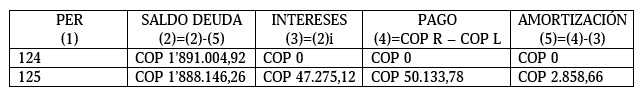
\includegraphics[trim=-78 -5 -78 -5]{7_Capitulo/img/ejemplos/5/5_2.jpg} }   \\ \hline
		\multicolumn{3}{|C{\textwidth}|}{
			$I_{58} =  308$.$678,20 \hspace{1mm} COP$ 

			$A =  84$.$591,05 \hspace{1mm} COP$
		}  \\ \hline
		
		
		%%%%%%%%%% FIN MATEMÁTICAS
		%%%%%% FIN RESPUESTA
	\end{longtable}
	%Se crean dos lineas en blanco para que no quede el siguiente texto tan pegado
	%\newline \newline %USARLO SI CREES QUE ES NECESARIO
\end{center}
%%%%%%%%%%%%%%%%%%%%%%%%%%FIN EJERCICIO 6B %%%%%%%%%%%%%%%%%%%%%%%%%%%
%%%%%%%%%%%%%%%%%%%%%%%%%%FIN EJERCICIO 6 %%%%%%%%%%%%%%%%%%%%%%%%%%%
	
	\section{Amortización mediante abono constante e interés anticipado}
	
	Una de las formas más difundidas de amortización consiste en cobrar intereses por anticipado y amortización constante al final de cada período, es de advertir que aquí, el pago periódico o cuota es variable, lo que es fijo es la amortización o abono a capital.Por tal motivo, la amortización puede calcularse dividiendo la deuda por el número de pagos a realizarse, esto es:
	\begin{center}
		$A=\frac{-VP}{n}$
	\end{center}
	Los intereses, por ser anticipados, se calculan aplicando la tasa al capital insoluto del mismo período y la cuota será igual a la amortización, mas los intereses. \\
	
	
	%%%%%%%%%%%%%%%%%%%%%%%%%%%%%%%%%%%%%%%%%%%%%%%%%%%%%%%%%%%%%%%%%%%%%%%%%%%%%%%%%%%%%%%%%%%%%%%%%%%%%%%%%%%%%%
	
	
\textbf{Ejemplo 7}\\
Una persona solicita a una entidad bancaria un préstamo por  COP  500.000. Lo cancelará en pagos trimestrales, durante un año, con amortización constante a capital e intereses del 33\% nominal anual trimestres anticipado. Elaborar una tabla de amortización.\\


%\newpage %USAR SOLO SI EL SOLUCIÓN QUEDA SOLO Y ES NECESARIO BAJARLO A LA SIGUIENTE PAGINA

\textbf{Solución 7}\\
%La tabla ira centrada
\begin{center}
	\renewcommand{\arraystretch}{1.5}% Margenes de las celdas
	%Creación de la cuadricula de 3 columnas
	\begin{longtable}[H]{|c|c|c|}
		%Creamos una linea horizontal
		\hline
		%Definimos el color de la primera fila
		\rowcolor[HTML]{FFB183}
		%%%%% INICIO ASIGNACIÓN período FOCAL %%%%%%%
		%%%%%%%%%% INICIO TITULO
		%Lo que se hace aquí es mezclar las 3 columnas en una sola
		\multicolumn{3}{|c|}{\cellcolor[HTML]{FFB183}\textbf{1. Asignación período focal}}   \\ \hline
		%%%%%%%%%% FIN TITULO
		%%%%% INICIO DECLARACIÓN DE VARIABLES %%%%%%%
		\multicolumn{3}{|c|}{$pf : 0 \textit{ pmv}$}\\ \hline
		%%%%%%%%%% INICIO TITULO
		%Lo que se hace aquí es mezclar las 3 columnas en una sola
		\multicolumn{3}{|c|}{\cellcolor[HTML]{FFB183}\textbf{2. Declaración de variables}}   \\ \hline
		%%%%%%%%%% FIN TITULO
		%%%%%%%%%% INICIO DE MATEMÁTICAS
		%Cada & hace referencia al paso de la siguiente columna
		\cellcolor[HTML]{FFB183}\textbf{Valores monetarios} & 
		\cellcolor[HTML]{FFB183}\textbf{Valores no monetarios} & 
		\cellcolor[HTML]{FFB183}\textbf{Incógnitas}  \\ \hline
	 	$ \hspace{1cm} VP= 500$.$000 \ COP \hspace{1cm}$ & $\hspace{1.5cm} i_a = 8.25\% \textit{ pta} \hspace{1.5cm}$ & $ R_1=\textit{?COP} $ \\
	 	& $\hspace{1.5cm} j_a = 33\% \textit{ nata} \hspace{1.5cm}$ & $ R_2=\textit{?COP} $ \\
	 	& $\hspace{1.5cm} n = 4 \textit{ pta} \hspace{1.5cm}$ & $ R_3=\textit{?COP} $ \\
	 	& $\hspace{1.5cm} A = \textit{ Constante} \hspace{1.5cm}$ & $ R_4=\textit{?COP} $ \\ \hline
		%%%%%%%%%% FIN DE MATEMÁTICAS
		%%%%% FIN DECLARACIÓN DE VARIABLES
		
		\rowcolor[HTML]{FFB183}
		\multicolumn{3}{|c|}{\cellcolor[HTML]{FFB183}\textbf{3. Diagrama de flujo de caja}} \\ \hline
		\multicolumn{3}{|c|}{ 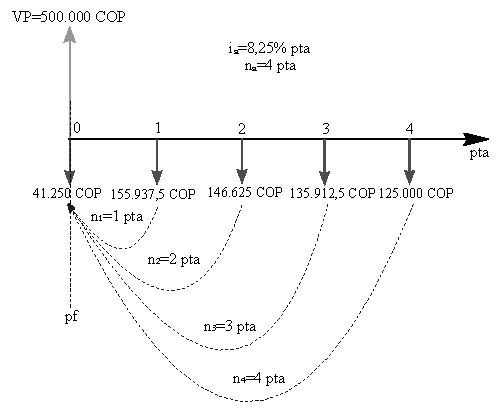
\includegraphics[trim=-78 -5 -78 -5]{7_Capitulo/img/ejemplos/7/7_1.pdf} }   \\ \hline
		%%%%% INICIO FLUJO DE CAJA
		\rowcolor[HTML]{FFB183}
		\multicolumn{3}{|c|}{\cellcolor[HTML]{FFB183}\textbf{4. Declaración de fórmulas}} \\ \hline
		%%%%%%%%%%%%% FIN INSERCIÓN DE IMAGEN
		%%%%%FIN FLUJO DE CAJA
		
		\multicolumn{3}{|c|}{ $ I = P i $ monto de intereses periódicos }   \\ 
		\multicolumn{3}{|c|}{ $ A = \frac{V P}{n} $ Amortización de capital iguales en n períodos, variará el monto de los intereses}   \\ 
		\multicolumn{3}{|c|}{ $R = A + I $  Valor de cuotas seriales fijas}   \\ \hline
		
		%%%%%% INICIO DESARROLLO MATEMÁTICO
		\rowcolor[HTML]{FFB183}
		%%%%%%%%%%INICIO TITULO
		\multicolumn{3}{|c|}{\cellcolor[HTML]{FFB183}\textbf{5. Desarrollo matemático}}       \\ \hline
		%%%%%%%%%% FIN TITULO
		%%%%%%%%%% INICIO MATEMÁTICAS
		\multicolumn{3}{|c|}{ $ A = \frac{500.000 }{4} \hspace{1mm} pta =  125$.$000 \hspace{1mm} COP$}   \\ 
		\multicolumn{3}{|c|}{ $R_{1} =   125$.$000 \hspace{1mm} COP  +  375$.$000( 0,0825) \hspace{1mm} COP$ }   \\ 
		\multicolumn{3}{|c|}{ $R_{1} =   155$.$937,50 \hspace{1mm} COP$ }   \\
		\multicolumn{3}{|c|}{ $R_{2} =   146$.$625 \hspace{1mm} COP$ }   \\
		\multicolumn{3}{|c|}{ $R_{3} =   135$.$912,50 \hspace{1mm} COP$ }   \\
		\multicolumn{3}{|c|}{ $R_{4} =   125$.$000 \hspace{1mm} COP$ }   \\ \hline
		
		%%%%%%%%%% FIN MATEMÁTICAS
		%%%%%% FIN DESARROLLO MATEMÁTICO
		%%%%%% INICIO RESPUESTA
		\rowcolor[HTML]{FFB183}
		%%%%%%%%%%INICIO TITULO
		\multicolumn{3}{|c|}{\cellcolor[HTML]{FFB183}\textbf{6. Respuesta}}   \\ \hline
		%%%%%%%%%% FIN TITULO
		%%%%%%%%%% INICIO RESPUESTA MATEMÁTICA
		\multicolumn{3}{|c|}{ 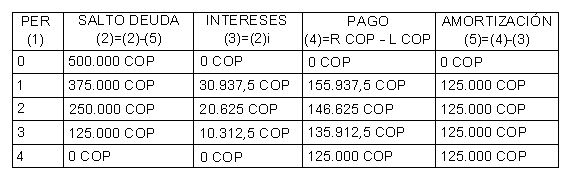
\includegraphics[trim=-78 -5 -78 -5]{7_Capitulo/img/ejemplos/7/7_2.pdf} }   \\ \hline
		
		
		%%%%%%%%%% FIN MATEMÁTICAS
		%%%%%% FIN RESPUESTA
	\end{longtable}
	%Se crean dos lineas en blanco para que no quede el siguiente texto tan pegado
	%\newline \newline %USARLO SI CREES QUE ES NECESARIO
\end{center}
%%%%%%%%%%%%%%%%%%%%%%%%%%FIN EJERCICIO 7 %%%%%%%%%%%%%%%%%%%%%%%%%%%
	%%%%%%%%%%%%%%%%%%%%%%%%%%%%%%%%%%%%%%%%%%%%%%%%%%%%%%%%%%%%%%%%%%%%%%%%%%%%%%%%%%%%%%%%%%%%%%%%%%%%%%%%%%%%%%

	%\newpage
	\section{Amortización mediante gradientes escalonados}
	Los sistemas escalonados pueden ser lineales o geométricos y éstos a su vez pueden ser crecientes o decrecientes; mediante éste sistema se logra \textbf{COMBINAR} cuotas constantes con cuotas crecientes o decrecientes. Es decir que conservaremos constante la cuota de amortización, durante un tiempo determinado, al final del cual se incrementa o decrementa, según el caso.\\\\
	Examinaremos dos situaciones, la primera será la \textbf{FUSIÓN} de una cuota constante con un \textbf{gradiente geométrico}; la segunda será la \textbf{FUSIÓN} de una cuota constante con un \textbf{gradiente lineal}; en ambos casos será necesario construir dos gráficas. La primera corresponde a la forma como se van a pagar las cuotas y en la segunda cada serie de cuotas iguales será reemplazada por una sola cuota al final del período. A la primera gráfica se le denominará gradiente escalonado y la segunda gráfica corresponde al gradiente simple.\\\\
	%Las definiciones que hemos dado con anterioridad continuarán vigentes para la segunda gráfica, pero para la primera gráfica a todas las definiciones se les antepondrá el prefijo inter o el prefijo sub, por tanto.
	El valor de cada pago lo denominaremos intercuota o subcuota y lo representaremos por \textbf{“r”} (minúscula), el tiempo que transcurre entre dos intercuotas lo denominaremos interperíodo y la tasa correspondiente al interperíodo se denominará intertasa o subtasa. Además, el número de intercuotas que hay por cada cuota es constante y se representará por "m" e indicará el tamaño del escalón, además, la altura del escalón vendrá dada por la diferencia que hay entre dos intercuotas cualesquiera pero de escalones contiguos y la representaremos por "H".\\\\
	%%%%%%%%%%%%%%%%%%%%%%%%%%%%%%%%%%%%%%%%%%%%%%%%%%%%%%%%%%%%%%%%%%%%%%%%%%%%%%%%%%%%%%%%%%%%%%%%%%%%%%%%%%%%%%%%%%%%%%%%%%%%%%%%%%%%%EJERCICIO 8 %%%%%%%%%%%%%%%%%%%%%%%%%%%
	%%%%%%%%%%%%%%%%%%%%%%%%%%%%%%%%%%%%%%%%%%%%%%%%%%%%%%%%%%%%%%%%%%%%%%%%%%%%%%%%%%%%%%%%%%%%%%%%%%%%%%%%%%%
%%%%%%%%%%%%%%%%%%%%%%%%%%EJERCICIO 8 %%%%%%%%%%%%%%%%%%%%%%%%%%%
	\textbf{Ejemplo 8}\\
	Elaborar una tabla para amortizar la suma de  300.000  COP, con un interés del 32\% nominal anual semestre vencido, mediante pagos semestrales, durante 3 años, bajo las siguientes condiciones:\\
	a)	la cuota anual aumenta en  60.000  COP \\
	b)	la intercuota aumenta en  25.000  COP  cada año \\
	c)	la intercuota aumenta un 25\% cada año\\\\
	
	%\newpage %USAR SOLO SI EL SOLUCIÓN QUEDA SOLO Y ES NECESARIO BAJARLO A LA SIGUIENTE PAGINA
	%%%%%%%%%%%%%%%%%%%%%%%%%%INICIO EJERCICIO 8a %%%%%%%%%%%%%%%%%%%%%%%%%%%
	%%%%%%%%%%%%%%%%%%%%%%%%%%INICIO EJERCICIO 8a %%%%%%%%%%%%%%%%%%%%%%%%%%%
\textbf{Solución a.}\\
% La tabla irá centrada
\begin{center}
	\renewcommand{\arraystretch}{1.5}% Márgenes de las celdas
	% Creación de la cuadrícula de 2 columnas
	\begin{longtable}[H]{|c|c|}
		% Creamos una línea horizontal
		\hline
		% Definimos el color de la primera fila
		\rowcolor[HTML]{FFB183} \hline
		%%%%% INICIO ASIGNACIÓN PERÍODO FOCAL %%%%%%%
		%%%%%%%%%% INICIO TÍTULO
		% Lo que se hace aquí es mezclar las 2 columnas en una sola
		\multicolumn{2}{|c|}{\cellcolor[HTML]{FFB183}\textbf{1. Asignación período focal}} \\ \hline
		%%%%%%%%%% FIN TÍTULO
		%%%%% INICIO DECLARACIÓN DE VARIABLES %%%%%%%
		\multicolumn{2}{|c|}{$pf : 0 \; \textit{psv}$} \\ \hline
		%%%%%%%%%% INICIO TÍTULO
		% Lo que se hace aquí es mezclar las 2 columnas en una sola
		\multicolumn{2}{|c|}{\cellcolor[HTML]{FFB183}\textbf{2. Declaración de variables}} \\ \hline

		%%%%%%%%%% FIN TÍTULO
		%%%%%%%%%% INICIO DE MATEMÁTICAS
		\cellcolor[HTML]{FFB183}\textbf{Valores monetarios} & 
		\cellcolor[HTML]{FFB183}\textbf{Valores no monetarios} \\ \hline
		$L = 60{.}000 \; \text{COP}$ & $j = 32\% \; \text{nasv}$ \\ 
		$H = 25{.}000 \; \text{COP}$ & $m = 2 \; \text{psv}$ \\ 
		$ $ & $n = 3 \; \text{pav}$ \\ \hline
		%%%%%%%%%% FIN DE MATEMÁTICAS
		%%%%% FIN DECLARACIÓN DE VARIABLES

		\rowcolor[HTML]{FFB183}
		\hline
		\multicolumn{2}{|c|}{\cellcolor[HTML]{FFB183}\textbf{3. Diagrama de flujo de caja}} \\ \hline
		\multicolumn{2}{|c|}{ 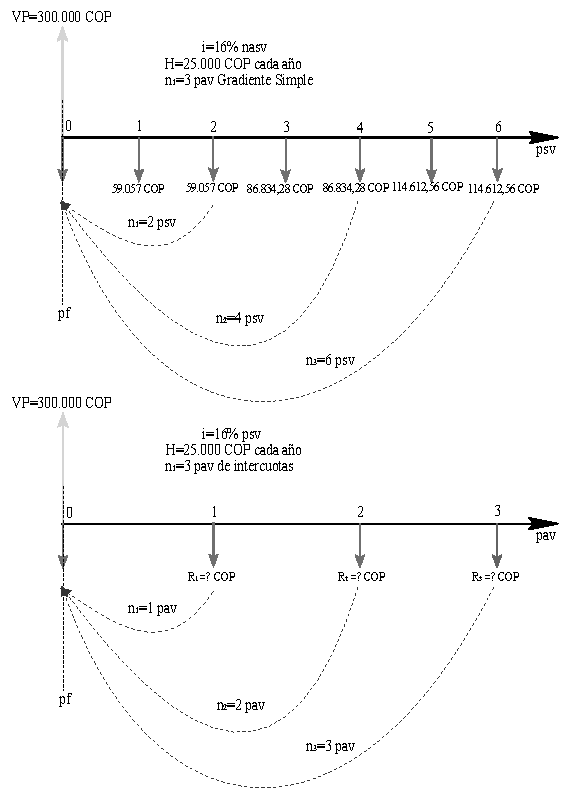
\includegraphics[trim=-78 -5 -78 -5]{7_Capitulo/img/ejemplos/8/8_1.pdf} } \\ \hline
		%%%%% INICIO FLUJO DE CAJA
		\rowcolor[HTML]{FFB183}
		\hline
		\multicolumn{2}{|c|}{\cellcolor[HTML]{FFB183}\textbf{4. Declaración de fórmulas}} \\ \hline
		%%%%%%%%%%%%% FIN INSERCIÓN DE IMAGEN
		%%%%% FIN FLUJO DE CAJA

		\multicolumn{2}{|c|}{ $(1 + i_{1})^{m_1} = (1 + i_{2})^{m_2}$ Equivalente de tasas periódicas vencidas } \\ 
		\multicolumn{2}{|c|}{ $VP = R \frac{1-(1+i)^{-n}}{i}$ Valor presente gradiente aritmético } \\ 
		\multicolumn{2}{|c|}{ $VP = \frac{(1+i)^{-n}-1}{i}$ Valor futuro de serie uniforme vencida } \\ 
		\multicolumn{2}{|c|}{ $R_{n} = R_{1} + (n -1)L$ Valor de un gradiente aritmético en un período \(n\)} \\ \hline

		%%%%%% INICIO DESARROLLO MATEMÁTICO
		\rowcolor[HTML]{FFB183}
		\hline
		%%%%%%%%%% INICIO TÍTULO
		\multicolumn{2}{|c|}{\cellcolor[HTML]{FFB183}\textbf{5. Desarrollo matemático}} \\ \hline
		%%%%%%%%%% FIN TÍTULO
		%%%%%%%%%% INICIO MATEMÁTICAS
		\multicolumn{2}{|c|}{ $(1 + 0{,}16)^{2} = (1 + i)^{1}$ } \\ 
		\multicolumn{2}{|c|}{ $i = 34{,}56\% \; \textit{pav}$ } \\ \hline

		%%%%%%%%%% FIN MATEMÁTICAS
		%%%%%% FIN DESARROLLO MATEMÁTICO
		%%%%%% INICIO RESPUESTA
		\rowcolor[HTML]{FFB183}
		\hline
		%%%%%%%%%% INICIO TÍTULO
		\multicolumn{2}{|c|}{\cellcolor[HTML]{FFB183}\textbf{6. Respuesta}} \\ \hline
		%%%%%%%%%% FIN TÍTULO
		%%%%%%%%%% INICIO RESPUESTA MATEMÁTICA
		\multicolumn{2}{|c|}{ 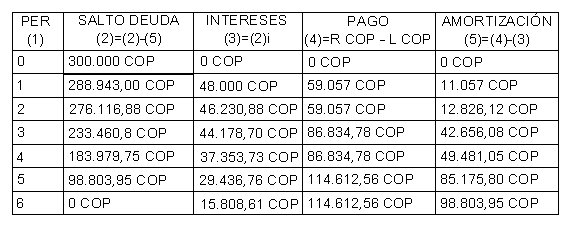
\includegraphics[trim=-78 -5 -78 -5]{7_Capitulo/img/ejemplos/8/8_1_1.pdf} } \\ \hline
	\end{longtable}
	% Se crean dos líneas en blanco para que no quede el siguiente texto tan pegado
	%\newline \newline % USARLO SI CREES QUE ES NECESARIO
\end{center}
%%%%%%%%%%%%%%%%%%%%%%%%%%FIN EJERCICIO 8a %%%%%%%%%%%%%%%%%%%%%%%%%%%

	%%%%%%%%%%%%%%%%%%%%%%%%%%FIN EJERCICIO 8a %%%%%%%%%%%%%%%%%%%%%%%%%%%
 
	%%%%%%%%%%%%%%%%%%%%%%%%%%EJERCICIO 8b %%%%%%%%%%%%%%%%%%%%%%%%%%%
	%%%%%%%%%%%%%%%%%%%%%%%%%%EJERCICIO 8b %%%%%%%%%%%%%%%%%%%%%%%%%%%
\textbf{Solución b.}\\
	%La tabla irá centrada
	\begin{center}
		\renewcommand{\arraystretch}{1.5}% Márgenes de las celdas
		% Creación de la cuadrícula de 2 columnas
		\begin{longtable}[H]{|c|c|}
			% Creamos una línea horizontal
			\hline
			% Definimos el color de la primera fila
			\rowcolor[HTML]{FFB183} 
			\hline
			%%%%% INICIO ASIGNACIÓN FECHA FOCAL %%%%%%%
			%%%%%%%%%% INICIO TÍTULO
			% Lo que se hace aquí es mezclar las 2 columnas en una sola
			\multicolumn{2}{|c|}{\cellcolor[HTML]{FFB183}\textbf{1. Asignación período focal}} \\ \hline
			%%%%%%%%%% FIN TÍTULO
			%%%%% INICIO DECLARACIÓN DE VARIABLES %%%%%%%
			\multicolumn{2}{|c|}{$pf : 0 \; \textit{psv}$} \\ \hline
			\hline
			%%%%%%%%%% INICIO TÍTULO
			% Lo que se hace aquí es mezclar las 2 columnas en una sola
			\multicolumn{2}{|c|}{\cellcolor[HTML]{FFB183}\textbf{2. Declaración de variables}} \\ \hline
			\hline 
			%%%%%%%%%% FIN TÍTULO
			%%%%%%%%%% INICIO DE MATEMÁTICAS
			% Cada & hace referencia al paso de la siguiente columna
			\cellcolor[HTML]{FFB183}\textbf{Valores monetarios} & 
			\cellcolor[HTML]{FFB183}\textbf{Valores no monetarios} \\ \hline
			$L = 60{.}000 \; \text{COP}$ & $m = 2 \; \textit{psv}$ \\ 
			$H = 25{.}000 \; \text{COP}$ & $n = 6 \; \textit{psv}$ \\ 
			$ $ & $i = 16\% \; \textit{psv}$ \\ \hline

			%%%%%%%%%% FIN DE MATEMÁTICAS
			%%%%% FIN DECLARACIÓN DE VARIABLES

			\rowcolor[HTML]{FFB183}
			\multicolumn{2}{|c|}{\cellcolor[HTML]{FFB183}\textbf{3. Diagrama de flujo de caja}} \\ \hline
			\multicolumn{2}{|c|}{ 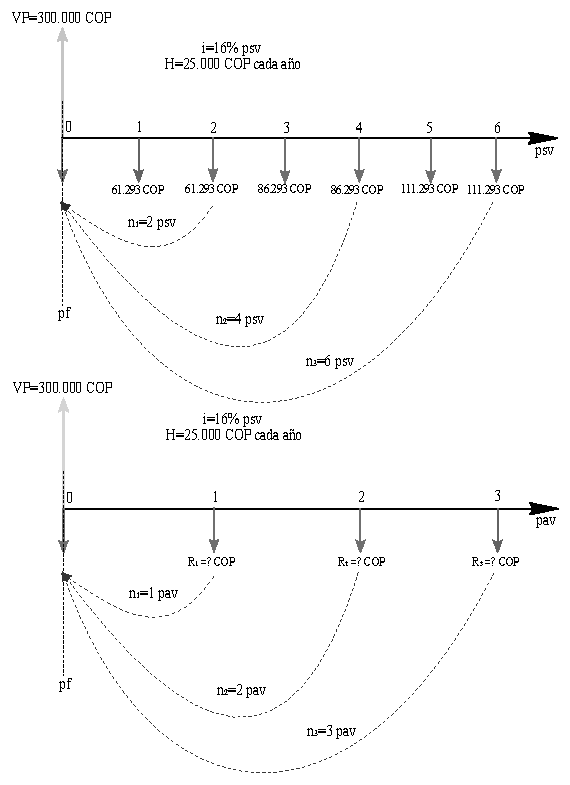
\includegraphics[trim=-78 -5 -78 -5]{7_Capitulo/img/ejemplos/8/8_2.pdf} } \\ \hline
			%%%%% INICIO FLUJO DE CAJA
			\rowcolor[HTML]{FFB183}
			\multicolumn{2}{|c|}{\cellcolor[HTML]{FFB183}\textbf{4. Declaración de fórmulas}} \\ \hline
			%%%%%%%%%%%%% FIN INSERCIÓN DE IMAGEN
			%%%%% FIN FLUJO DE CAJA

			\multicolumn{2}{|c|}{ $VP = R \frac{1-(1+i)^{-n}}{i} $ Valor presente de serie uniforme vencida } \\ 
			\multicolumn{2}{|c|}{ $VF = \frac{(1+i)^{-n}-1}{i} $ Valor futuro de serie uniforme vencida } \\ \hline
			
			%%%%%% INICIO DESARROLLO MATEMÁTICO
			\rowcolor[HTML]{FFB183}
			%%%%%%%%%% INICIO TÍTULO
			\multicolumn{2}{|c|}{\cellcolor[HTML]{FFB183}\textbf{5. Desarrollo matemático}} \\ \hline
			%%%%%%%%%% FIN TÍTULO
			%%%%%%%%%% INICIO MATEMÁTICAS
			\multicolumn{2}{|c|}{ $ L = \frac{ 25{.}000 \; \text{COP} (1 + 0{.}16)^{2} - 1}{0{.}16} = 54{.}000 \; \text{COP}$ } \\ 
			\multicolumn{2}{|c|}{ $ r_{1} = r_{2} = 61{.}293{,}00 \; \text{COP} $ } \\ \hline

			%%%%%%%%%% FIN MATEMÁTICAS
			%%%%%% FIN DESARROLLO MATEMÁTICO
			%%%%%% INICIO RESPUESTA
			\rowcolor[HTML]{FFB183}
			%%%%%%%%%% INICIO TÍTULO
			\multicolumn{2}{|c|}{\cellcolor[HTML]{FFB183}\textbf{6. Respuesta}} \\ \hline
			%%%%%%%%%% FIN TÍTULO
			%%%%%%%%%% INICIO RESPUESTA MATEMÁTICA
			\multicolumn{2}{|c|}{ 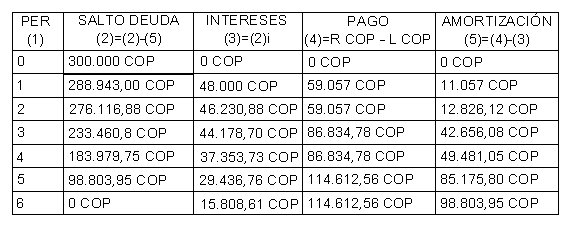
\includegraphics[trim=-78 -5 -78 -5]{7_Capitulo/img/ejemplos/8/8_2_2.pdf} } \\ \hline
		\end{longtable}
	\end{center}
%%%%%%%%%%%%%%%%%%%%%%%%%%FIN EJERCICIO 8b %%%%%%%%%%%%%%%%%%%%%%%%%%%

	%%%%%%%%%%%%%%%%%%%%%%%%%%FIN EJERCICIO 8b %%%%%%%%%%%%%%%%%%%%%%%%%%%
 
	%%%%%%%%%%%%%%%%%%%%%%%%%%EJERCICIO 8c %%%%%%%%%%%%%%%%%%%%%%%%%%%
    %%%%%%%%%%%%%%%%%%%%%%%%%%EJERCICIO 8c %%%%%%%%%%%%%%%%%%%%%%%%%%%
\textbf{Solución c.}\\
	%La tabla irá centrada
	\begin{center}
		\renewcommand{\arraystretch}{1.5}% Márgenes de las celdas
		% Creación de la cuadrícula de 1 columna
		\begin{longtable}[H]{|c|}
			% Creamos una línea horizontal
			\hline
			% Definimos el color de la primera fila
			\rowcolor[HTML]{FFB183}
			\hline
			%%%%% INICIO ASIGNACIÓN FECHA FOCAL %%%%%%%
			%%%%%%%%%% INICIO TÍTULO
			% Lo que se hace aquí es mezclar la columna en una sola
			\multicolumn{1}{|c|}{\cellcolor[HTML]{FFB183}\textbf{1. Asignación período focal}} \\ \hline
			%%%%%%%%%% FIN TÍTULO
			%%%%% INICIO DECLARACIÓN DE VARIABLES %%%%%%%
			\multicolumn{1}{|c|}{$pf : 0 \; \textit{psv}$} \\ \hline
			\hline
			%%%%%%%%%% INICIO TÍTULO
			% Lo que se hace aquí es mezclar la columna en una sola
			\multicolumn{1}{|c|}{\cellcolor[HTML]{FFB183}\textbf{2. Declaración de variables}} \\ \hline
			\cellcolor[HTML]{FFB183}\textbf{Valores no monetarios} \\ \hline
			%%%%%%%%%% FIN TÍTULO
			%%%%%%%%%% INICIO DE MATEMÁTICAS
			$m = 2 \; \textit{psv}$ \\ 
			$g = 25\%$ \\ 
			$n = 3 \; \textit{pav}$ \\ 
			$i = 34,56\% \; \textit{pav}$ \\ \hline
			%%%%%%%%%% FIN DE MATEMÁTICAS
			%%%%% FIN DECLARACIÓN DE VARIABLES

			\rowcolor[HTML]{FFB183}
			\hline
			\multicolumn{1}{|c|}{\cellcolor[HTML]{FFB183}\textbf{3. Diagrama de flujo de caja}} \\ \hline
			\multicolumn{1}{|c|}{ 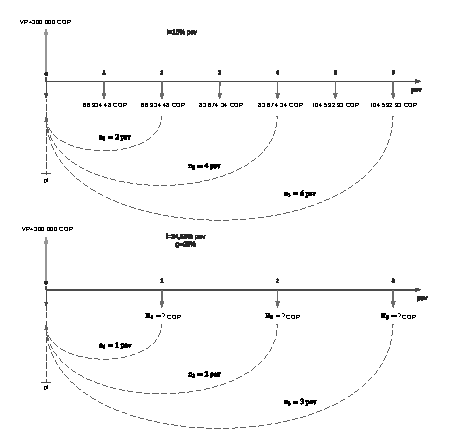
\includegraphics[trim=-78 -5 -78 -5,width=17cm]{7_Capitulo/img/ejemplos/8/8_3.pdf} } \\ \hline
			%%%%% INICIO FLUJO DE CAJA
			\rowcolor[HTML]{FFB183}
			\hline
			\multicolumn{1}{|c|}{\cellcolor[HTML]{FFB183}\textbf{4. Declaración de fórmulas}} \\ \hline
			%%%%%%%%%%%%% FIN INSERCIÓN DE IMAGEN
			%%%%% FIN FLUJO DE CAJA

			\multicolumn{1}{|c|}{ $VP = \frac{R( (1 + g)^{n} (1+i)^{-n} - 1)}{g-i} $ Valor presente gradiente geométrico } \\ \hline
			
			%%%%%% INICIO DESARROLLO MATEMÁTICO
			\rowcolor[HTML]{FFB183}
			\hline
			%%%%%%%%%% INICIO TÍTULO
			\multicolumn{1}{|c|}{\cellcolor[HTML]{FFB183}\textbf{5. Desarrollo matemático}} \\ \hline
			%%%%%%%%%% FIN TÍTULO
			%%%%%%%%%% INICIO MATEMÁTICAS
			\multicolumn{1}{|c|}{ $300{.}000 \; \text{COP} = \frac{R_{1}( (1 + 0{.}25)^{3} (1+0{.}3456)^{-3} - 1)}{0{.}25-0{.}3456} $ } \\ 
			\multicolumn{1}{|c|}{ $R_{1} = 225{.}920{,}73 \; \text{COP} $ } \\ \hline

			%%%%%%%%%% FIN MATEMÁTICAS
			%%%%%% FIN DESARROLLO MATEMÁTICO
			%%%%%% INICIO RESPUESTA
			\rowcolor[HTML]{FFB183}
			\hline
			%%%%%%%%%% INICIO TÍTULO
			\multicolumn{1}{|c|}{\cellcolor[HTML]{FFB183}\textbf{6. Respuesta}} \\ \hline
			%%%%%%%%%% FIN TÍTULO
			%%%%%%%%%% INICIO RESPUESTA MATEMÁTICA
			\multicolumn{1}{|c|}{ 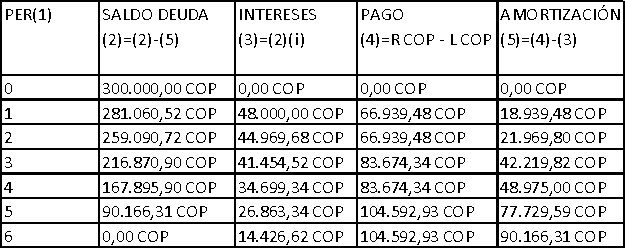
\includegraphics[trim=-78 -5 -78 -5]{7_Capitulo/img/ejemplos/8/8_3_3.pdf} } \\ \hline
		\end{longtable}
	\end{center}
%%%%%%%%%%%%%%%%%%%%%%%%%%FIN EJERCICIO 8c %%%%%%%%%%%%%%%%%%%%%%%%%%%

    %%%%%%%%%%%%%%%%%%%%%%%%%%FIN EJERCICIO 8c %%%%%%%%%%%%%%%%%%%%%%%%%%%

%%%%%%%%%%%%%%%%%%%%%%%%%%FIN EJERCICIO 8 %%%%%%%%%%%%%%%%%%%%%%%%%%%
	%%%%%%%%%%%%%%%%%%%%%%%%%%FIN EJERCICIO 8 %%%%%%%%%%%%%%%%%%%%%%%%%%%%%%%%%%%%%%%%%%%%%%%%%%%%%%%%%%%%%%%%%%%%%%%%%%%%%%%%%%%%%%%%%%%%%%%%%%%%%%%
	
	
	%%%%%%%%%%%%%%%%%%%%%%%%%%%%%%%%%%%%%%%%%%%%%%%%%%%%%%%%%%%%%%%%%%%%%%%%%%%%%%%%%%%%%%%%%%%%%%%%%%%%%%%%%%%%%%%%%%%%%%%%%%%%%%%%%%%%%EJERCICIO 9 %%%%%%%%%%%%%%%%%%%%%%%%%%%
	%%%%%%%%%%%%%%%%%%%%%%%%%%EJERCICIO 9 %%%%%%%%%%%%%%%%%%%%%%%%%%%
\textbf{Ejemplo 9}\\
Amortizar en valor constante la suma de 500{.}000 COP mediante 3 pagos anuales que decrecen en 20{.}000 COP; suponga un interés del 10\% periódico anual vencido y una tasa única de corrección monetaria del 24\% nominal anual año vencido.\\			
				
\textbf{Solución 9}\\
% La tabla irá centrada
\begin{center}
	\renewcommand{\arraystretch}{1.5}% Márgenes de las celdas
	% Creación de la cuadrícula de 3 columnas
	\begin{longtable}[H]{|c|c|c|}
		% Creamos una línea horizontal
		\hline
		% Definimos el color de la primera fila
		\rowcolor[HTML]{FFB183}
		\hline
		%%%%% INICIO ASIGNACIÓN PERÍODO FOCAL %%%%%%%
		%%%%%%%%%% INICIO TÍTULO
		% Lo que se hace aquí es mezclar las 3 columnas en una sola
		\multicolumn{3}{|c|}{\cellcolor[HTML]{FFB183}\textbf{1. Asignación período focal}} \\ \hline
		%%%%%%%%%% FIN TÍTULO
		%%%%% INICIO DECLARACIÓN DE VARIABLES %%%%%%%
		\multicolumn{3}{|c|}{$pf : 0 \; \textit{pav}$} \\ \hline
		%%%%%%%%%% INICIO TÍTULO
		% Lo que se hace aquí es mezclar las 3 columnas en una sola
		\multicolumn{3}{|c|}{\cellcolor[HTML]{FFB183}\textbf{2. Declaración de variables}} \\ \hline
		%%%%%%%%%% FIN TÍTULO
		%%%%%%%%%% INICIO DE MATEMÁTICAS
		\cellcolor[HTML]{FFB183}\textbf{Valores monetarios} & 
		\cellcolor[HTML]{FFB183}\textbf{Valores no monetarios} & 
		\cellcolor[HTML]{FFB183}\textbf{Incógnitas} \\ \hline
		$VP = 500{.}000 \; \text{COP}$ & $n = 3 \; \textit{pav}$ & $R_{1} = ? \; \text{COP}$ \\ 
		$L = -20{.}000 \; \text{COP}$ & $i = 10\% \; \textit{pav}$ & $R_{2} = ? \; \text{COP}$ \\ 
		$ $ & $ $ & $R_{3} = ? \; \text{COP}$ \\ \hline
		%%%%%%%%%% FIN DE MATEMÁTICAS
		%%%%% FIN DECLARACIÓN DE VARIABLES

		\rowcolor[HTML]{FFB183}
		\hline
		\multicolumn{3}{|c|}{\cellcolor[HTML]{FFB183}\textbf{3. Diagrama de flujo de caja}} \\ \hline
		\multicolumn{3}{|c|}{ 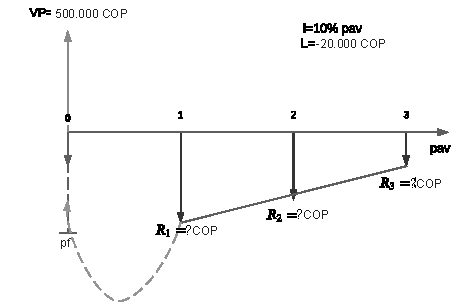
\includegraphics[trim=-78 -5 -78 -5]{7_Capitulo/img/ejemplos/9/9_1.pdf} } \\ \hline
		%%%%% INICIO FLUJO DE CAJA
		\rowcolor[HTML]{FFB183}
		\hline
		\multicolumn{3}{|c|}{\cellcolor[HTML]{FFB183}\textbf{4. Declaración de fórmulas}} \\ \hline
		%%%%%%%%%%%%% FIN INSERCIÓN DE IMAGEN
		%%%%% FIN FLUJO DE CAJA

		\multicolumn{3}{|c|}{ $VP = R\frac{1- (1+i)^{-n} }{i} + \frac{L}{i} \left( \frac{1- (1+i)^{-n} }{i} - n(1+i)^{-n}\right) $ Valor presente serie uniforme anticipada } \\ \hline
		
		%%%%%% INICIO DESARROLLO MATEMÁTICO
		\rowcolor[HTML]{FFB183}
		\hline
		%%%%%%%%%% INICIO TÍTULO
		\multicolumn{3}{|c|}{\cellcolor[HTML]{FFB183}\textbf{5. Desarrollo matemático}} \\ \hline
		%%%%%%%%%% FIN TÍTULO
		%%%%%%%%%% INICIO MATEMÁTICAS
		\multicolumn{3}{|c|}{ $500{.}000 \; \text{COP} = R\frac{1- (1+0{.}10)^{-3} }{0{.}10} + \frac{-20{.}000}{0{.}10} \left( \frac{1- (1+0{.}10)^{-3} }{0{.}10} - 3(1+0{.}10)^{-3}\right) $ } \\ 
		\multicolumn{3}{|c|}{ $R = 219{.}788{,}52 \; \text{COP}$ } \\ 
		\multicolumn{3}{|c|}{ $R_{1} = 219{.}788{,}52 \; \text{COP} \cdot (1 + 0{.}24)^{1} = 272{.}537{,}76 \; \text{COP}$ } \\ 
		\multicolumn{3}{|c|}{ $R_{2} = 199{.}788{,}52 \; \text{COP} \cdot (1 + 0{.}24)^{2} = 307{.}194{,}83 \; \text{COP}$ } \\ 
		\multicolumn{3}{|c|}{ $R_{3} = 179{.}788{,}52 \; \text{COP} \cdot (1 + 0{.}24)^{3} = 342{.}789{,}12 \; \text{COP}$ } \\ \hline
	
		%%%%%%%%%% FIN MATEMÁTICAS
		%%%%%% FIN DESARROLLO MATEMÁTICO
		%%%%%% INICIO RESPUESTA
		\rowcolor[HTML]{FFB183}
		\hline
		%%%%%%%%%% INICIO TÍTULO
		\multicolumn{3}{|c|}{\cellcolor[HTML]{FFB183}\textbf{6. Respuesta}} \\ \hline
		%%%%%%%%%% FIN TÍTULO
		%%%%%%%%%% INICIO RESPUESTA MATEMÁTICA
		\multicolumn{3}{|c|}{ 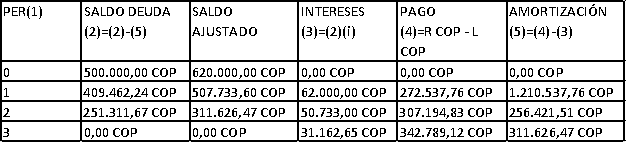
\includegraphics[trim=-78 -5 -78 -5]{7_Capitulo/img/ejemplos/9/9_2.pdf} } \\ \hline
	\end{longtable}
	% Se crean dos líneas en blanco para que no quede el siguiente texto tan pegado
	%\newline \newline % USARLO SI CREES QUE ES NECESARIO
\end{center}
%%%%%%%%%%%%%%%%%%%%%%%%%%FIN EJERCICIO 9 %%%%%%%%%%%%%%%%%%%%%%%%%%%

	%%%%%%%%%%%%%%%%%%%%%%%%%%FIN EJERCICIO 9 %%%%%%%%%%%%%%%%%%%%%%%%%%%
	
	
	%%%%%%%%%%%%%%%%%%%%%%%%%%EJERCICIO 10 %%%%%%%%%%%%%%%%%%%%%%%%%%%
    %%%%%%%%%%%%%%%%%%%%%%%%%%EJERCICIO 10 %%%%%%%%%%%%%%%%%%%%%%%%%%%
\textbf{Ejemplo 10}\\
Resolver el problema anterior, suponiendo que el gradiente es escalonado con pagos semestrales.\\		

\textbf{Solución 10}\\
% La tabla irá centrada
\begin{center}
	\renewcommand{\arraystretch}{1.5}% Márgenes de las celdas
	% Creación de la cuadrícula de 2 columnas
	\begin{longtable}[H]{|c|c|}
		% Creamos una línea horizontal
		\hline
		% Definimos el color de la primera fila
		\rowcolor[HTML]{FFB183}
		\hline
		%%%%% INICIO ASIGNACIÓN PERÍODO FOCAL %%%%%%%
		%%%%%%%%%% INICIO TÍTULO
		% Lo que se hace aquí es mezclar las 2 columnas en una sola
		\multicolumn{2}{|c|}{\cellcolor[HTML]{FFB183}\textbf{1. Asignación período focal}} \\ \hline
		%%%%%%%%%% FIN TÍTULO
		%%%%% INICIO DECLARACIÓN DE VARIABLES %%%%%%%
		\multicolumn{2}{|c|}{$pf : 0 \; \textit{psv}$} \\ \hline
		%%%%%%%%%% INICIO TÍTULO
		% Lo que se hace aquí es mezclar las 2 columnas en una sola
		\multicolumn{2}{|c|}{\cellcolor[HTML]{FFB183}\textbf{2. Declaración de variables}} \\ \hline
		%%%%%%%%%% FIN TÍTULO
		%%%%%%%%%% INICIO DE MATEMÁTICAS
		\cellcolor[HTML]{FFB183}\textbf{Valores monetarios} & 
		\cellcolor[HTML]{FFB183}\textbf{Valores no monetarios} \\ \hline
		$VP = 500{.}000 \; \text{COP}$ & $n_{1} = 1 \; \textit{psv}$ \\ 
		$ $ & $n_{2} = 2 \; \textit{psv}$ \\ 
		$ $ & $n_{3} = 3 \; \textit{psv}$ \\ 
		$ $ & $n_{5} = 5 \; \textit{psv}$ \\ 
		$ $ & $n_{6} = 6 \; \textit{psv}$ \\ 
		$ $ & $i = 11{,}3552\% \; \textit{psv}$ \\ \hline
		%%%%%%%%%% FIN DE MATEMÁTICAS
		%%%%% FIN DECLARACIÓN DE VARIABLES

		\rowcolor[HTML]{FFB183}
		\hline
		\multicolumn{2}{|c|}{\cellcolor[HTML]{FFB183}\textbf{3. Diagrama de flujo de caja}} \\ \hline
		\multicolumn{2}{|c|}{ 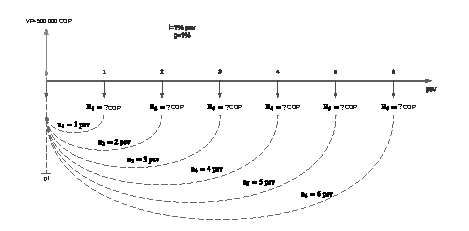
\includegraphics[trim=-78 -5 -78 -5]{7_Capitulo/img/ejemplos/10/10_1.pdf} } \\ \hline
		%%%%% INICIO FLUJO DE CAJA
		\rowcolor[HTML]{FFB183}
		\hline
		\multicolumn{2}{|c|}{\cellcolor[HTML]{FFB183}\textbf{4. Declaración de fórmulas}} \\ \hline
		%%%%%%%%%%%%% FIN INSERCIÓN DE IMAGEN
		%%%%% FIN FLUJO DE CAJA

		\multicolumn{2}{|c|}{ $(1+i_1)^{m_1} = (1+i_2)^{m_2} $ Equivalencia de tasas } \\  
		\multicolumn{2}{|c|}{ $VF = R\frac{(1+i)^{n} -1 }{i} $ Valor presente serie uniforme } \\ \hline
		
		%%%%%% INICIO DESARROLLO MATEMÁTICO
		\rowcolor[HTML]{FFB183}
		\hline
		%%%%%%%%%% INICIO TÍTULO
		\multicolumn{2}{|c|}{\cellcolor[HTML]{FFB183}\textbf{5. Desarrollo matemático}} \\ \hline
		%%%%%%%%%% FIN TÍTULO
		%%%%%%%%%% INICIO MATEMÁTICAS
		\multicolumn{2}{|c|}{ $(1+ 0{.}24)^{1} = (1+i)^{2}$ } \\ 
		\multicolumn{2}{|c|}{ $i = 11{,}3552\% \; \textit{psv}$ } \\ \hline

		%%%%%%%%%% FIN MATEMÁTICAS
		%%%%%% FIN DESARROLLO MATEMÁTICO
		%%%%%% INICIO RESPUESTA
		\rowcolor[HTML]{FFB183}
		\hline
		%%%%%%%%%% INICIO TÍTULO
		\multicolumn{2}{|c|}{\cellcolor[HTML]{FFB183}\textbf{6. Respuesta}} \\ \hline
		%%%%%%%%%% FIN TÍTULO
		%%%%%%%%%% INICIO RESPUESTA MATEMÁTICA
		\multicolumn{2}{|c|}{ 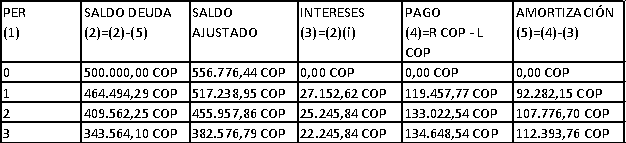
\includegraphics[trim=-78 -5 -78 -5]{7_Capitulo/img/ejemplos/10/10_2.pdf} } \\ \hline
	\end{longtable}
	% Se crean dos líneas en blanco para que no quede el siguiente texto tan pegado
	%\newline \newline % USARLO SI CREES QUE ES NECESARIO
\end{center}
%%%%%%%%%%%%%%%%%%%%%%%%%%FIN EJERCICIO 10 %%%%%%%%%%%%%%%%%%%%%%%%%%%

	%%%%%%%%%%%%%%%%%%%%%%%%%%FIN EJERCICIO 10 %%%%%%%%%%%%%%%%%%%%%%%%%%%
	
	
	\section{Capitalización diferida (*)}
	Se entiende por capitalización diferida a la capitalización que tiene uno o varios períodos en los cuales no se efectúan depósitos, pero el capital ahorrado si gana intereses. Es obvio que estos períodos se encontrarán entre la fecha del último depósito y la fecha de retiro del capital. \\
	
	
	%\textbf{Ejemplo 17}\\
	
	%%%%%%%%%%%%%%%%%%%%%%%%%%EJERCICIO 11 %%%%%%%%%%%%%%%%%%%%%%%%%%%%%%%%%%%%%%%%%%%%%%%%%%%%%%
	%%%%%%%%%%%%%%%%%%%%%%%%%%EJERCICIO 11 %%%%%%%%%%%%%%%%%%%%%%%%%%%
\textbf{Ejemplo 11}\\
Para el día 15 de abril de 1998 debe haberse reunido la suma de 900{.}000 COP. Para tal fin, se efectúan depósitos trimestrales de \(R \; \text{COP}\) c/u en un fondo que paga el 32\% nominal anual trimestre vencido. Si el primer depósito se hace el 15 de enero de 1997 y el último el 15 de octubre de 1997, calcular el valor del depósito trimestral y elaborar una tabla de capitalización.\\		

\textbf{Solución 11}\\
% La tabla irá centrada
\begin{center}
	\renewcommand{\arraystretch}{1.5}% Márgenes de las celdas
	% Creación de la cuadrícula de 3 columnas
	\begin{longtable}[H]{|c|c|c|}
		% Creamos una línea horizontal
		\hline
		% Definimos el color de la primera fila
		\rowcolor[HTML]{FFB183}
		\hline
		%%%%% INICIO ASIGNACIÓN PERÍODO FOCAL %%%%%%%
		%%%%%%%%%% INICIO TÍTULO
		% Lo que se hace aquí es mezclar las 3 columnas en una sola
		\multicolumn{3}{|c|}{\cellcolor[HTML]{FFB183}\textbf{1. Asignación período focal}} \\ \hline
		%%%%%%%%%% FIN TÍTULO
		%%%%% INICIO DECLARACIÓN DE VARIABLES %%%%%%%
		\multicolumn{3}{|c|}{$pf : 7 \; \textit{ptv}$} \\ \hline
		\hline
		%%%%%%%%%% INICIO TÍTULO
		% Lo que se hace aquí es mezclar las 3 columnas en una sola
		\multicolumn{3}{|c|}{\cellcolor[HTML]{FFB183}\textbf{2. Declaración de variables}} \\ \hline
		%%%%%%%%%% FIN TÍTULO
		%%%%%%%%%% INICIO DE MATEMÁTICAS
		\hline
		\cellcolor[HTML]{FFB183}\textbf{Valores monetarios} & 
		\cellcolor[HTML]{FFB183}\textbf{Valores no monetarios} & 
		\cellcolor[HTML]{FFB183}\textbf{Incógnitas} \\ \hline
		$VF = 900{.}000 \; \text{COP}$ & $n = 4 \; \textit{ptv}$ & $R = ? \; \text{COP}$ \\ 
		$ $ & $j = 32\% \; \textit{natv}$ & \\ 
		$ $ & $i = 8\% \; \textit{ptv}$ & \\ \hline
		%%%%%%%%%% FIN DE MATEMÁTICAS
		%%%%% FIN DECLARACIÓN DE VARIABLES

		\rowcolor[HTML]{FFB183}
		\hline
		\multicolumn{3}{|c|}{\cellcolor[HTML]{FFB183}\textbf{3. Diagrama de flujo de caja}} \\ \hline
		\multicolumn{3}{|c|}{ 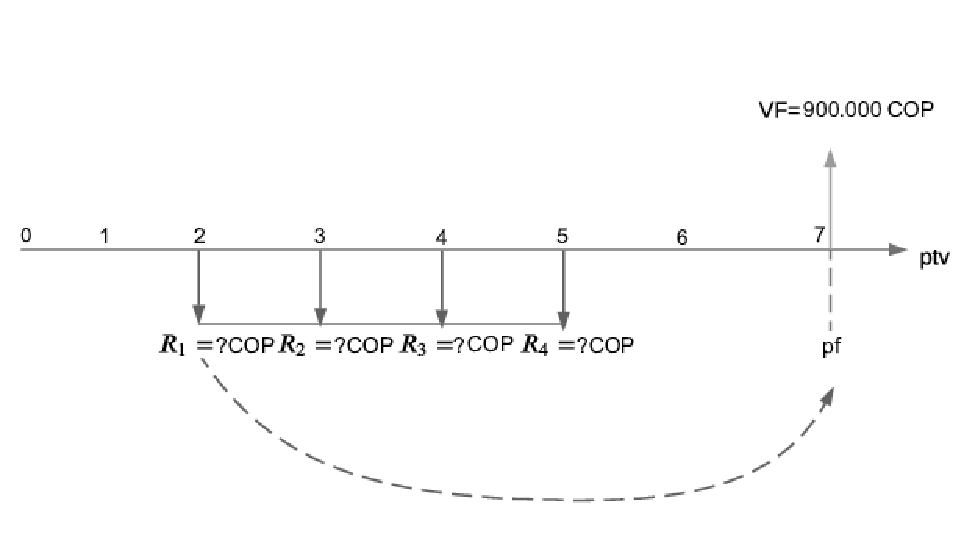
\includegraphics[trim=-78 -5 -78 -5, width=14cm]{7_Capitulo/img/ejemplos/11/11_1.pdf} } \\ \hline
		%%%%% INICIO FLUJO DE CAJA
		\rowcolor[HTML]{FFB183}
		\hline
		\multicolumn{3}{|c|}{\cellcolor[HTML]{FFB183}\textbf{4. Declaración de fórmulas}} \\ \hline
		%%%%%%%%%%%%% FIN INSERCIÓN DE IMAGEN
		%%%%% FIN FLUJO DE CAJA

		\multicolumn{3}{|c|}{ $VF = R_{n}(1+i)^{n-1}$ Valor futuro de un Gradiente Geométrico si \(g = i\) } \\ \hline
		
		%%%%%% INICIO DESARROLLO MATEMÁTICO
		\rowcolor[HTML]{FFB183}
		\hline
		%%%%%%%%%% INICIO TÍTULO
		\multicolumn{3}{|c|}{\cellcolor[HTML]{FFB183}\textbf{5. Desarrollo matemático}} \\ \hline
		%%%%%%%%%% FIN TÍTULO
		%%%%%%%%%% INICIO MATEMÁTICAS
		\multicolumn{3}{|c|}{ $900{.}000 \; \text{COP} = R_{4} (1 + 0{.}08)^{2}$ } \\ 
		\multicolumn{3}{|c|}{ $R = 171{.}235{,}19 \; \text{COP}$ } \\ \hline

		%%%%%%%%%% FIN MATEMÁTICAS
		%%%%%% FIN DESARROLLO MATEMÁTICO
		%%%%%% INICIO RESPUESTA
		\rowcolor[HTML]{FFB183}
		\hline
		%%%%%%%%%% INICIO TÍTULO
		\multicolumn{3}{|c|}{\cellcolor[HTML]{FFB183}\textbf{6. Respuesta}} \\ \hline
		%%%%%%%%%% FIN TÍTULO
		%%%%%%%%%% INICIO RESPUESTA MATEMÁTICA
		\multicolumn{3}{|c|}{ 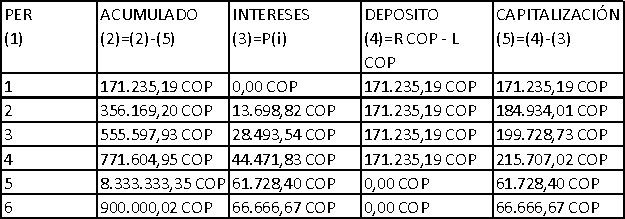
\includegraphics[trim=-78 -5 -78 -5]{7_Capitulo/img/ejemplos/11/11_2.pdf} } \\ \hline
	\end{longtable}
	% Se crean dos líneas en blanco para que no quede el siguiente texto tan pegado
	%\newline \newline % USARLO SI CREES QUE ES NECESARIO
\end{center}
%%%%%%%%%%%%%%%%%%%%%%%%%%FIN EJERCICIO 11 %%%%%%%%%%%%%%%%%%%%%%%%%%%

	%%%%%%%%%%%%%%%%%%%%%%%%%%FIN EJERCICIO 11 %%%%%%%%%%%%%%%%%%%%%%%%%%%%%%%%%%%%%%%%%%%%%%%%%%%%%%%%%%%%%%%%%%%%%%%%%%%%%%%%%%%%%%%%%%%%%%%%%%%%%%%%%%%%
	
	Observación: el error de  0.02 COP se debe a la aproximación en el valor de la cuota.\\
	
	\section{Capitalización por cuotas con reliquidación de intereses}
	
	Las bases teóricas necesarias para elaborar la tabla son las mismas de la amortización pero poniendo la ecuación en valor final, en consecuencia no entraremos en más detalles.\\
	
	
	
	
	 %%%%%%%%%%%%%%%%%%%%%%%%%%%%%%%%%%%%%%%%%%%%%%%%%%%%%%%%%%%%%%%%%%%%%%%%%%%%%%%%%%%%%%%%%%%%%%%%%%%%%%%%%%%%%%%%%%%%%%%%%%%%%%%%%%%%%%EJERCICIO 12 %%%%%%%%%%%%%%%%%%%%%%%%%%%%%%%%%%%%%%%%%%%%%%%%%%%%%%
	%%%%%%%%%%%%%%%%%%%%%%%%%%EJERCICIO 12 %%%%%%%%%%%%%%%%%%%%%%%%%%%
\textbf{Ejemplo 12}\\
Se desean reunir 800{.}000 \; \text{COP} en 4 depósitos periódicos trimestre vencido crecientes en un 20\% más una cuota extra pactada de 80{.}000 \; \text{COP} en el período 2 trimestre vencido. Con una tasa del 20\% período trimestre vencido. Elabore la tabla de capitalización.\\

\textbf{Solución 12}\\
% La tabla irá centrada
\begin{center}
	\renewcommand{\arraystretch}{1.5}% Márgenes de las celdas
	% Creación de la cuadrícula de 3 columnas
	\begin{longtable}[H]{|c|c|c|}
		% Creamos una línea horizontal
		\hline
		% Definimos el color de la primera fila
		\rowcolor[HTML]{FFB183}
		\hline
		%%%%% INICIO ASIGNACIÓN PERÍODO FOCAL %%%%%%%
		%%%%%%%%%% INICIO TÍTULO
		% Lo que se hace aquí es mezclar las 3 columnas en una sola
		\multicolumn{3}{|c|}{\cellcolor[HTML]{FFB183}\textbf{1. Asignación período focal}} \\ \hline
		%%%%%%%%%% FIN TÍTULO
		%%%%% INICIO DECLARACIÓN DE VARIABLES %%%%%%%
		\multicolumn{3}{|c|}{$pf : 5 \; \textit{ptv}$} \\ \hline
		%%%%%%%%%% INICIO TÍTULO
		% Lo que se hace aquí es mezclar las 3 columnas en una sola
		\multicolumn{3}{|c|}{\cellcolor[HTML]{FFB183}\textbf{2. Declaración de variables}} \\ \hline
		\hline
		%%%%%%%%%% FIN TÍTULO
		%%%%%%%%%% INICIO DE MATEMÁTICAS
		\cellcolor[HTML]{FFB183}\textbf{Valores monetarios} & 
		\cellcolor[HTML]{FFB183}\textbf{Valores no monetarios} & 
		\cellcolor[HTML]{FFB183}\textbf{Incógnitas} \\ \hline
		$VF = 800{.}000 \; \text{COP}$ & $g = 20\%$ & $R_{1} = ? \; \text{COP}$ \\ 
		$R = 80{.}000 \; \text{COP}$ & $n = 4 \; \textit{ptv}$ & \\ 
		$ $ & $i = 20\% \; \textit{ptv}$ & \\ \hline
		%%%%%%%%%% FIN DE MATEMÁTICAS
		%%%%% FIN DECLARACIÓN DE VARIABLES

		\rowcolor[HTML]{FFB183}
		\hline
		\multicolumn{3}{|c|}{\cellcolor[HTML]{FFB183}\textbf{3. Diagrama de flujo de caja}} \\ \hline
		\multicolumn{3}{|c|}{ 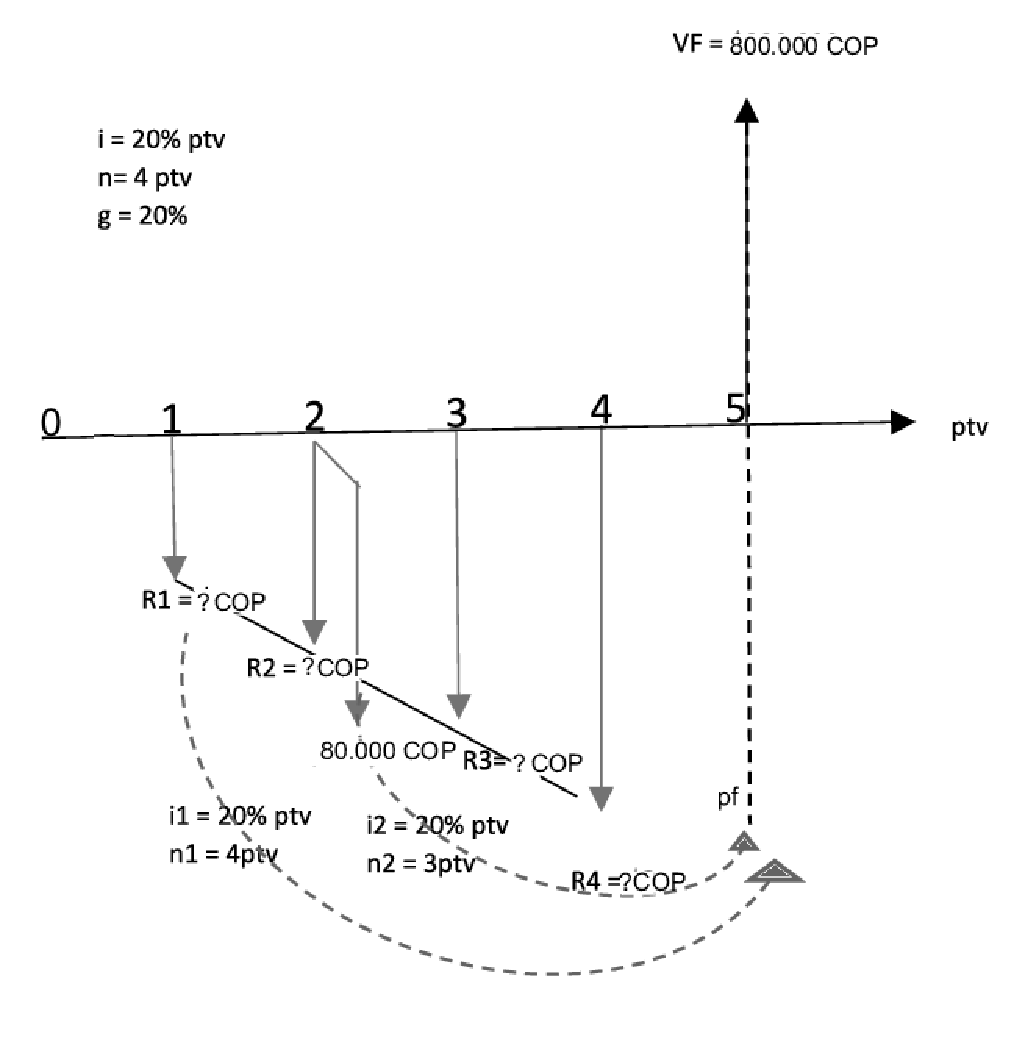
\includegraphics[trim=-78 -5 -78 -5, width=14cm]{7_Capitulo/img/ejemplos/12/12_1.pdf} } \\ \hline
		%%%%% INICIO FLUJO DE CAJA
		\rowcolor[HTML]{FFB183}
		\hline
		\multicolumn{3}{|c|}{\cellcolor[HTML]{FFB183}\textbf{4. Declaración de fórmulas}} \\ \hline
		%%%%%%%%%%%%% FIN INSERCIÓN DE IMAGEN
		%%%%% FIN FLUJO DE CAJA

		\multicolumn{3}{|c|}{ $VF = R_{1} n (1+i)^{n-1} + R (1+i)^{2}$ Valor futuro de un Gradiente Geométrico } \\ \hline
		
		%%%%%% INICIO DESARROLLO MATEMÁTICO
		\rowcolor[HTML]{FFB183}
		\hline
		%%%%%%%%%% INICIO TÍTULO
		\multicolumn{3}{|c|}{\cellcolor[HTML]{FFB183}\textbf{5. Desarrollo matemático}} \\ \hline
		%%%%%%%%%% FIN TÍTULO
		%%%%%%%%%% INICIO MATEMÁTICAS
		\multicolumn{3}{|c|}{ $800{.}000 \; \text{COP} = R_{1} \cdot 4 \cdot (1 + 0{.}2)^{3} + 80{.}000 \; \text{COP} \cdot (1 + 0{.}2)^{2}$ } \\ 
		\multicolumn{3}{|c|}{ $R_{1} = 99{.}074{,}07 \; \text{COP}$ } \\ 
		\multicolumn{3}{|c|}{ $R_{2} = 99{.}074{,}07 \; \text{COP} \cdot (1 + 0{.}2)^{1} + 80{.}000 \; \text{COP} = 198{.}888{,}89 \; \text{COP}$ } \\ 
		\multicolumn{3}{|c|}{ $R_{3} = 99{.}074{,}07 \; \text{COP} \cdot (1 + 0{.}2)^{2} = 142{.}666{,}67 \; \text{COP}$ } \\ 
		\multicolumn{3}{|c|}{ $R_{4} = 99{.}074{,}07 \; \text{COP} \cdot (1 + 0{.}2)^{3} = 171{.}200{,}00 \; \text{COP}$ } \\ \hline

		%%%%%%%%%% FIN MATEMÁTICAS
		%%%%%% FIN DESARROLLO MATEMÁTICO
		%%%%%% INICIO RESPUESTA
		\rowcolor[HTML]{FFB183}
		\hline
		%%%%%%%%%% INICIO TÍTULO
		\multicolumn{3}{|c|}{\cellcolor[HTML]{FFB183}\textbf{6. Respuesta}} \\ \hline
		%%%%%%%%%% FIN TÍTULO
		%%%%%%%%%% INICIO RESPUESTA MATEMÁTICA
		\multicolumn{3}{|c|}{ 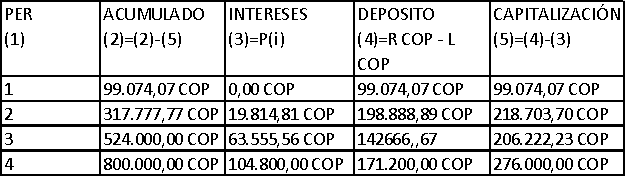
\includegraphics[trim=-78 -5 -78 -5]{7_Capitulo/img/ejemplos/12/12_2.pdf} } \\ \hline
	\end{longtable}
	% Se crean dos líneas en blanco para que no quede el siguiente texto tan pegado
	%\newline \newline % USARLO SI CREES QUE ES NECESARIO
\end{center}
%%%%%%%%%%%%%%%%%%%%%%%%%%FIN EJERCICIO 12 %%%%%%%%%%%%%%%%%%%%%%%%%%%

	%%%%%%%%%%%%%%%%%%%%%%%%%%FIN EJERCICIO 12 %%%%%%%%%%%%%%%%%%%%%%%%%%%%%%%%%%%%%%%%%%%%%%%%%%%%%%%%%%%%%%%%%%%%%%%%%%%%%%%%%%%%%%%%%%%%%%%%%%%%%%%%%%%%
	
	
	
	\section{Costo periódico de una deuda}
	
	Cuando el fondo está destinado a cancelar una deuda y los depósitos en el fondo son uniformes entonces se denomina costo periódico de una deuda a la cantidad que debemos disponer en cada período para pagar los intereses de la deuda y hacer el depósito correspondiente en el fondo. Según la duración del período, se dice que la deuda tiene un costo trimestral, mensual, etc.\\
	
	\begin{comment}
	\textbf{Ejemplo 19}\\
	Supongamos que tenemos que pagar la suma de  COP  800.000 al final de 2 años y mientras tanto debemos pagar intereses a la tasa del 3\% mensual vencido. Con el fin de ir reuniendo el dinero necesario para cancelar la deuda se constituye un fondo mediante depósitos mensuales iguales que ganan un interés del 2.5\% efectivo mensual. Calcular el costo mensual de la deuda.\\
	
	\textbf{Solución:}\\
	\textbf{a.}	Diagrama de flujo de caja:
	\begin{center}
		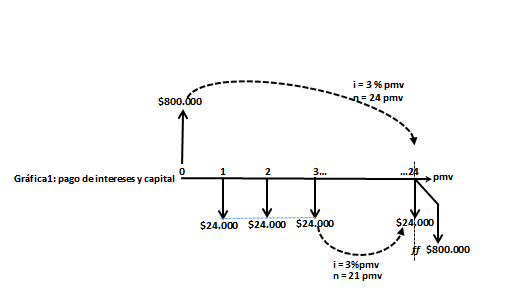
\includegraphics[height=9cm]{7_48}
	\end{center}
	\\
	\begin{center}
		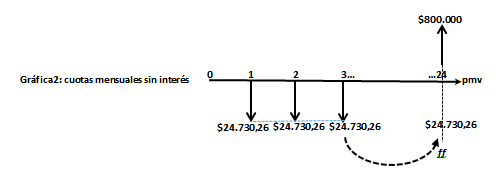
\includegraphics[height=6cm]{7_49}
	\end{center}
	
	Mensualmente debemos pagar un interés de  COP  800.000 x 0,03 =  COP  24.000
	Por otra parte, el depósito mensual en el fondo será:
	 COP  800.000 = Rx24 (1,025); \\R =   COP  24.730,26
	Y el costo mensual de la deuda será: 24.000 + 24.730,26 =  COP  48.730,26\\
	
	\textbf{b.}	Respuesta:\\
	La primera gráfica representa el pago de intereses y la deuda, la segunda gráfica representa los depósitos en el fondo y el capital reunido, al final de los 2 años se cancela el fondo y con ese dinero se paga la deuda.\\
	
	\textbf{Observación:} cuando la capitalización se hace mediante cuotas crecientes, por ejemplo con un gradiente, entonces el costo de la deuda de cada período es variable.\\
	\end{comment}
	%\textbf{Ejemplo 20}\\
	
	%%%%%%%%%%%%%%%%%%%%%%%%%%%%%%%%%%%%%%%%%%%%%%%%%%%%%%%%%%%%%%%%%%%%%%%%%%%%%%%%%%%%%%%%%%%%%%%%%%%%%%%%%%%%
	
	%%%%%%%%%%%%%%%%%%%%%%%%%%EJERCICIO 13 %%%%%%%%%%%%%%%%%%%%%%%%%%%%%%%%%%%%%%%%%%%%%%%%%%%%%%
		%%%%%%%%%%%%%%%%%%%%%%%%%%EJERCICIO 13 %%%%%%%%%%%%%%%%%%%%%%%%%%%%%%%%%%%%%%%%%%%%%%%%%%%%%%
    \textbf{Ejemplo 13}\\
	
	Una cuota inicial del 30\% y el saldo será pagadero al final de 3 años, mientras tanto se pagarán intereses por período mes anticipado al 3\%. Con el objeto de cancelar la deuda a su vencimiento, se constituye un fondo que paga el 33\% nominal anual mes vencido mediante depósitos mensuales ordinarios crecientes en 2.000 COP. Determinar el costo del período 15.\\
	
	\textbf{Solución 13}\\
	%La tabla ira centrada
	\begin{center}
		\renewcommand{\arraystretch}{1.5}% Margenes de las celdas
		%Creación de la cuadricula de 3 columnas
		\begin{longtable}[H]{|p{0.5\linewidth}|p{0.5\linewidth}|}
			%Creamos una linea horizontal
			\hline
			%Definimos el color de la primera fila
			\rowcolor[HTML]{FFB183}
			%%%%% INICIO ASIGNACIÓN período FOCAL %%%%%%%
			%%%%%%%%%% INICIO TITULO
			%Lo que se hace aquí es mezclar las 3 columnas en una sola
			\multicolumn{2}{|c|}{\cellcolor[HTML]{FFB183}\textbf{1. Asignación período focal}}   \\ \hline
			%%%%%%%%%% FIN TITULO
			%%%%% INICIO DECLARACIÓN DE VARIABLES %%%%%%%
			\multicolumn{2}{|c|}{$pf : 36 \textit{ pmv}$}\\ \hline
			%%%%%%%%%% INICIO TITULO
			%Lo que se hace aquí es mezclar las 3 columnas en una sola
			\multicolumn{2}{|c|}{\cellcolor[HTML]{FFB183}\textbf{2. Declaración de variables}}   \\ \hline
			%%%%%%%%%% FIN TITULO
			%%%%%%%%%% INICIO DE MATEMÁTICAS
			%Cada & hace referencia al paso de la siguiente columna
			\cellcolor[HTML]{FFB183}\textbf{Valores monetarios} & 
			\cellcolor[HTML]{FFB183}\textbf{Valores no monetarios} \\ \hline
			$Interés = 4{.}200{.}000 \; \text{COP} \cdot 0{,}03 = 126{.}000 \; \text{COP}$ & $n = 36 \; \textit{pmv}$ \\ 
			$ $ & $i = 3\% \; \textit{pmv}$ \\ \hline
			%%%%%%%%%% FIN DE MATEMÁTICAS
			%%%%% FIN DECLARACIÓN DE VARIABLES
			
			\rowcolor[HTML]{FFB183}
			\multicolumn{2}{|c|}{\cellcolor[HTML]{FFB183}\textbf{3. Diagrama de flujo de caja}} \\ \hline
			\multicolumn{2}{|c|}{ 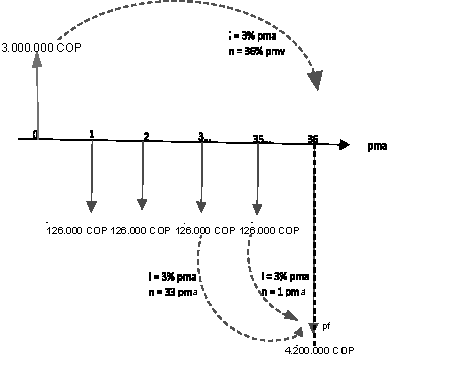
\includegraphics[trim=-78 -5 -78 -5]{7_Capitulo/img/ejemplos/13/13_1.pdf} }   \\
			\multicolumn{2}{|c|}{ 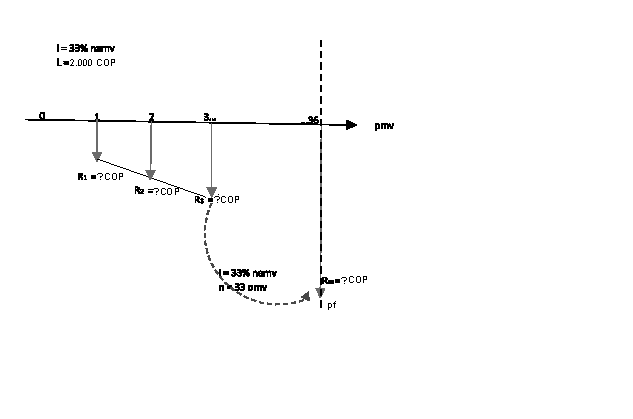
\includegraphics[trim=-78 -5 -78 -5]{7_Capitulo/img/ejemplos/13/13_2.pdf} }   \\ \hline
			%%%%% INICIO FLUJO DE CAJA
			\rowcolor[HTML]{FFB183}
			\multicolumn{2}{|c|}{\cellcolor[HTML]{FFB183}\textbf{4. Declaración de fórmulas}} \\ \hline
			%%%%%%%%%%%%% FIN INSERCIÓN DE IMAGEN
			%%%%%FIN FLUJO DE CAJA
			\multicolumn{2}{|c|}{ $VF = R n(1+i)^{n-1} $ \hspace{1mm} Formula del valor futuro gradiente geométrico si g=i}\\    
			\multicolumn{2}{|c|}{ $R_{n} = R_{1} + (n-1)L $ \hspace{1mm} Valor de un periodo aritmetico en un periodo n}   \\ \hline
			
			%%%%%% INICIO DESARROLLO MATEMÁTICO
			\rowcolor[HTML]{FFB183}
			%%%%%%%%%%INICIO TITULO
			\multicolumn{2}{|c|}{\cellcolor[HTML]{FFB183}\textbf{5. Desarrollo matemático}}       \\ \hline
			%%%%%%%%%% FIN TITULO
			%%%%%%%%%% INICIO MATEMÁTICAS
			\multicolumn{2}{|c|}{  $ 4.200.000 \ COP = R_{1} (36) (0,0275) + \frac{ 2.000 \ COP }{0,0275} ((36)(0,0275)-36) $}   \\ 
			\multicolumn{2}{|c|}{  $  R_{1} = 40.531,73 \ COP $}   \\ 
			\multicolumn{2}{|c|}{ $  R_{15} = 40.531,73 \ COP +  ( 15 - 1) (2.000 \ COP) = 68.531,73 \ COP $}   \\  \hline
			
			%%%%%%%%%% FIN MATEMÁTICAS
			%%%%%% FIN DESARROLLO MATEMÁTICO
			%%%%%% INICIO RESPUESTA
			\rowcolor[HTML]{FFB183}
			%%%%%%%%%%INICIO TITULO
			\multicolumn{2}{|c|}{\cellcolor[HTML]{FFB183}\textbf{6. Respuesta}}   \\ \hline
			%%%%%%%%%% FIN TITULO
			%%%%%%%%%% INICIO RESPUESTA MATEMÁTICA
			%\multicolumn{2}{|c|}{ 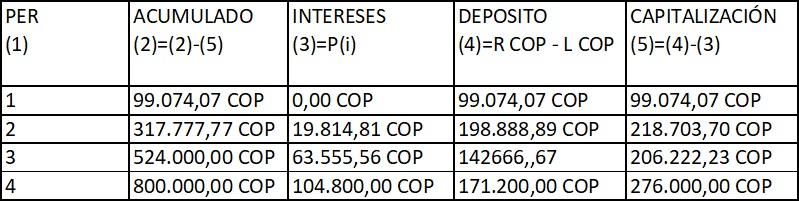
\includegraphics[trim=-78 -5 -78 -5]{7_Capitulo/img/ejemplos/12/12_2.jpg} }   \\ \hline
			\multicolumn{2}{|C{\textwidth}|}{
				$  R_{1} = 40.531,73 \ COP \hspace{2mm} y  \hspace{2mm} R_{15} = 68.531,73 \ COP $
				
				Esto significa que en el período 15 el deudor debe disponer de 194.531,73 COP de los cuales 126.000 COP los dedica al pago de intereses y el resto (68.531,73 COP) se deposita en el fondo.
				
			}  \\ \hline
			
			
			%%%%%%%%%% FIN MATEMÁTICAS
			%%%%%% FIN RESPUESTA
		\end{longtable}
		%Se crean dos lineas en blanco para que no quede el siguiente texto tan pegado
		%\newline \newline %USARLO SI CREES QUE ES NECESARIO
	\end{center}
%%%%%%%%%%%%%%%%%%%%%%%%%%FIN EJERCICIO 13
	%%%%%%%%%%%%%%%%%%%%%%%%%%FIN EJERCICIO 13
	
	
